\documentclass[utf8, zavrsni, numeric]{fer}
\usepackage{booktabs}
\usepackage{tabularx}
\usepackage{natbib}
\usepackage{float}
\usepackage{listings}
\usepackage{graphicx}
\usepackage{subfig}

\begin{document}

\nocite{*}

\thesisnumber{5118}

\title{Gusta stereoskopska rekonstrukcija poluglobalnim podudaranjem}

\author{Nikola Bunjevac}

\maketitle

% Ispis stranice s napomenom o umetanju izvornika rada. Uklonite naredbu \izvornik ako želite izbaciti tu stranicu.
\izvornik

\zahvala{Zahvaljujem se mentoru prof.~dr.~sc.~Siniši~Šegviću na pomoći pri izradi ovog rada
te svojoj obitelji na podršci tijekom cijelog školovanja}

\tableofcontents

\chapter{Uvod}
Računalni vid iznimno je zanimljivo interdisciplinarno područje koje se svrstava kao grana umjetne inteligencije.
Ono se bavi omogućavanjem računalima da shvate i interpretiraju podatke iz digitalnih slika i videozapisa.
Vid je jedno od najznačajnijih osjetila jer pomoću njega primamo mnoštvo korisnih informacija.
Pomoću vida se orijentiramo u prostoru, prepoznajemo druge ljude i njihova lica, čitamo, prikupljamo informacije itd.
Kada bi računala mogla interpretirati vizualne podražaje poput ljudi, to bi omogućilo velik
napredak u umjetnoj inteligenciji. Nažalost, to je još uvijek neriješen problem.

Samo područje
je nastalo šezdesetih godina prošlog stoljeća kada se mislilo da će se taj problem relativno brzo riješiti.
Naime, profesor je kao zadatak studentu zadao da na robota stavi kameru i da robot opisuje ono što vidi.
Vrlo brzo se pokazalo kako je problem puno složeniji nego što se mislilo.
S druge strane, od tada su ostvareni veliki napretci u tom području kao i općenito u umjetnoj inteligenciji.

U ovom radu ćemo opisati neke metode za stvaranje rekonstrukcije dubine prostora iz slika dviju kamera. Takvi sustavi se nazivaju stereo sustavi, a takva vrsta vida stereo vid.
Oni funkcioniraju analogno ljudskom vidu koji se još naziva binokularni vid zbog toga što ljudi gledaju pomoću dva oka. To ljudima omogućava stvaranje vrlo kvalitetnog dojma o 3D osobinama prostora kojega promatraju. Mogu zaključiti koliko je nešto udaljeno, odnos veličina raznih predmeta itd.

Gusta stereoskopska rekonstrukcija pokušava iz dvaju slika rekonstruirati gusti oblak točaka koji
odgovara prostoru koji se promatra. Postupak se odvija u nekoliko koraka.
Prvo je potrebno obraditi slike kako bi se otklonile fizičke nesavršenosti sustava poput nesavršenosti leće i položaja senzora. Zatim je potrebno piksele
transformirati kako bi svi korespondentni pikseli ležali na istom pravcu, odnosno epipolarnoj liniji. Nakon toga se može krenuti u rekonstrukciju scene.

Postoje dvije glavne podjele metoda guste stereoskopske rekonstrukcije, a to su
\begin{enumerate}
  \item lokalne metode i
  \item globalne metode.
\end{enumerate}

Lokalne metode se temelje na promatranju lokalne okoline svakog pojedinog piksela koju ćemo nazvati prozorčić.
Postupak rekonstrukcije tada se svodi na traženje najsličnijeg prozorčića na drugoj slici. Važno je naglasiti kako se traženje vrši samo duž epipolarne linije.
Za razliku od lokalnih, globalne metode rekonstrukciju rade pomoću svih piksela slike što intuitivno dovodi do zaključka da je postupak složeniji i zahtijeva više računalnih resursa.

Metoda poluglobalnog podudaranja, koju ćemo detaljnije obrađivati u ovom radu, može se svrstati negdje između. Naime, ona kao ulaz prima izračunate korespondencije lokalnih metoda, a zatim radi optimizaciju nad pikselima duž iste linije u osam ili šesnaest smjerova.
Takva optimizacije dovodi do kvalitetnijih rezultata u dijelovima gdje dolazi do nagle promjene u dubini scene.

U sljedećem poglavlju ćemo ukratko objasniti postupke kalibracije stereo sustava te rektifikacije parova slika kao predradnja postupku rekonstrukcije.

U trećem poglavlju ćemo obraditi nekoliko lokalnih metoda guste stereoskopske rekonstrukcije. Lokalne metode nude relativno dobre rezultate uz prihvatljivu performansu.

Zatim ćemo definirati algoritam poluglobalnog podudaranja, razraditi njegove hiperparametre te vidjeti kakva poboljšanja nudi u odnosu na lokalne metode.

Sljedeće poglavlje opisuje implementaciju navedenih algoritama i pomoćnih skripti te daje kratke upute za korištenje.

U petom poglavlju ćemo vidjeti rezultate eksperimenata na standardnim skupovima slika, usporedbe obrađenih metoda i komentare, nakon čega slijedi zaključak.

\chapter{Stereoskopska rekonstrukcija}

Prije same rekonstrukcije, potrebno je obraditi slike dobivene iz para kamera. Za to je potrebno znati geometrijske parametre sustava dvaju kamera. Kao model kamere uzet ćemo
projekcijsku ravninu koja je udaljena od izvora/kamere za neku udaljenost $f$. Tako se sve točke u prostoru ispred kamere i ravnine projiciraju na tu zamišljenu ravninu.

\begin{figure}[htb]
  \centering
  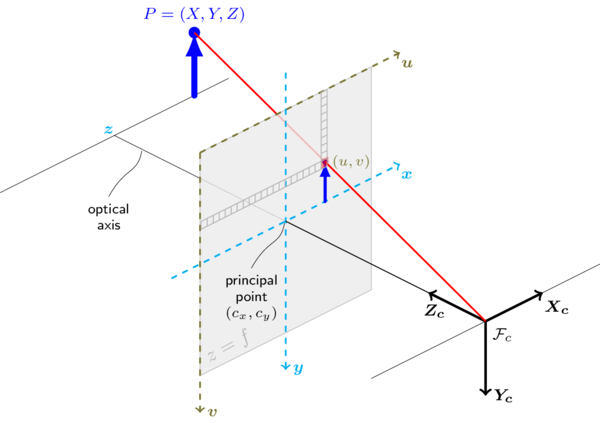
\includegraphics[width=13cm]{img/pinhole_camera_model.png}
  \caption{Model kamere (preuzeto iz dokumentacije biblioteke OpenCV)}
  \label{fig:model-kamere}
\end{figure}

Na slici \ref{fig:model-kamere} prikazan je upravo takav model. Kamera se nalazi u ishodištu
globalnog koordinatnog sustava s osima $(X_c, Y_c, Z_c)$. Ispred kamere u smjeru pozitivne
$Z$ osi na udaljenosti $z = f$ nalazi se projekcijska ravnina okomita na navedenu os. Udaljenost $f$ još se naziva žarišna udaljenost (eng. {\sl focal distance}). Koordinatni sustav projekcijske ravnine
ili slike određen osima $(u, v)$ je smješten tako da mu je ishodište u gornjem lijevom kutu slike.

Postupak stvaranja slike si možemo predočiti tako da zamislimo da za svaki piksel slike ispucamo
zraku koja ide iz globalnog ishodišta (kamere), prolazi kroz ravninu projekcije i ide sve dok ne pogodi neki najbliži vidljivi predmet. Boju u pogođenoj točki preslikavamo na ravninu projekciju, i to u točki sjecišta ispucane zrake i ravnine.

Naravno, ovo je vrlo rudimentaran model i u stvarnosti je postupak puno kompleksniji jer nismo
uzeli u obzir valna svojstva svjetlosti već smo pretpostavili da se svjetlost širi pravocrtno.

\section{Epipolarna geometrija}

Geometrijske parametre sustava kamera možemo podijeliti u dvije skupine:
\begin{enumerate}
  \item intrinzični parametri
  \item ekstrinzični parametri.
\end{enumerate}

Intrinzični parametri su svojstveni svakoj kameri pojedinačno, dok su im ekstrinzični parametri zajednički. Neka svojstva koja utječu na intrinzične parametre su nesavršenost leće (radijalna distorzija, slika \ref{fig:primjeri-distorzije}), pomak senzora
od centra leće (tangencijalna distorzija) i slične fizičke nesavršenosti koje je ponekad nemoguće izbjeći. Stoga priskačemo programskom otklanjanju tih nedostataka.
Ekstrinzični parametri dovode do transformacija kako bismo slike doveli u istu ravninu projekcije te postigli da svi pikseli duž horizontalnog pravca jedne slike odgovaraju istom pravcu (na istoj visini) na drugoj slici.
Taj pravac se naziva epipolarna linija. Razlog takvih transformacija je olakšavanje traženja korespondentnih točaka koje sada treba tražiti samo duž epipolarne linije čime je problem sveden na jednu dimenziju. Vidimo da uz malo pretprocesiranja puno olakšavamo problem rekonstrukcije.

\begin{figure}[htb]
  \centering
  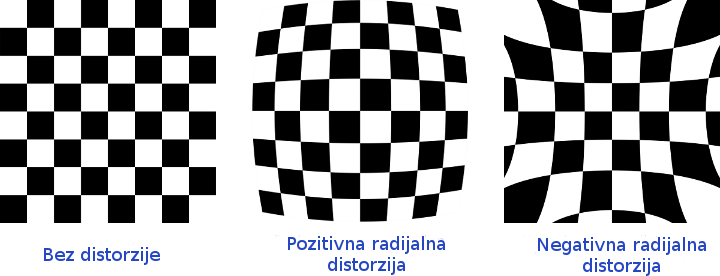
\includegraphics[width=13cm]{img/distortion_examples.png}
  \caption{Primjeri distorzije (preuzeto iz dokumentacije biblioteke OpenCV)}
  \label{fig:primjeri-distorzije}
\end{figure}

\section{Rektifikacija}
Postupak rektifikacije odgovara transformaciji slika kako bismo dobili slike koje zadovoljavaju gore navedena svojstva, a to su:
\begin{enumerate}
  \item Pikseli koji odgovaraju točkama u prostoru na istoj visini nalaze se duž iste epipolarne linije
  \item Nema distorzije uzrokovane lećom
  \item Projekcijske ravnine leže u istoj ravnini
\end{enumerate}
Za rektifikaciju su potrebni ekstrinzični parametri sustava kamera, a za izračun ekstrinzičnih parametara su potrebni intrinzični.
Nakon provedenih transformacija intriznični parametri obaju kamera su jednaki (npr. imaju istu žarišnu udaljenost što je lako predočiti kada znamo da projekcije sada leže u istoj ravnini te je svaka točka
u prostoru ispred jednako udaljena od oba projekcijska platna).

Ovaj postupak se obično provodi uz pomoć šahovske ploče koja je pogodna za to zbog svojih svojstava. Potrebno je parom kamera uslikati dovoljan broj slika na kojima se u potpunosti vidi šahovnica.
Nakon toga se mogu odrediti ranije navedeni parametri. Postupak se odvija u nekoliko koraka, od kojih je prvi traženje šahovskih polja. Nakon toga se pomoću kuteva iz uglova polja može odrediti distorzija
i ostali parametri.

Navedene postupke implementira i nudi biblioteka OpenCV \footnote{http://opencv.org/}. Korisno je istaknuti kako je u korištenim skupovima slika postupak kalibracije i rektifikacije već proveden, barem u skupovima za treniranje. Moguće je doći i do nerektificiranih, sirovih slika pa sam provesti navedene postupke.

\begin{figure}[htb]
  \centering
  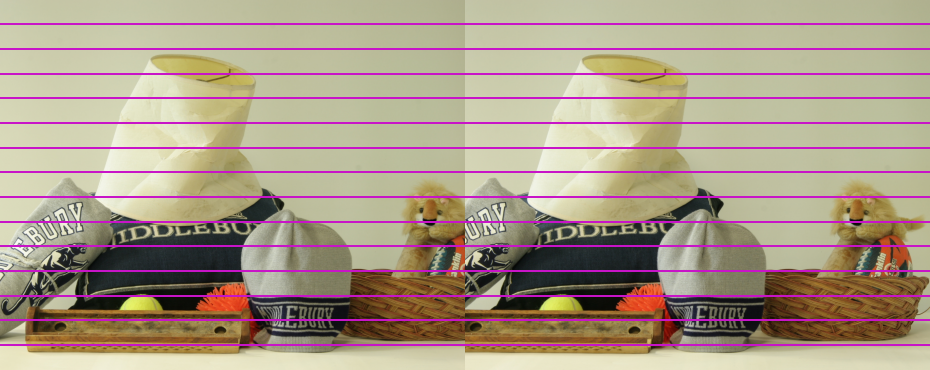
\includegraphics[width=14cm]{img/lines.png}
  \caption{Prikaz epipolarnih linija}
  \label{fig:epipolarne_linije}
\end{figure}

Na slici \ref{fig:epipolarne_linije} su prikazane dvije slike iz skupa Middlebury na kojima
se vide epipolarne linije. Možemo primijetiti kako iste točke u prostoru leže na istim epipolarnim
linijama. To je upravo svojstvo koje smo htjeli dobiti rektifikacijom parova slika lijeve i desne kamere.
Sada možemo lako uvidjeti zašto je korespondentne piksele potrebno tražiti samo duž iste $y$-koordinate.

\section{Rekonstrukcija udaljenosti}
Sada ćemo opisati postupak za rekonstrukciju udaljenosti pojedinih točaka u prostoru od kamere. Taj postupak se još naziva i trijangulacija. Izračun se temelji na disparitetima određenim prilikom stereoskopske rekonstrukcije.
Stanje je prikazano na slici \ref{fig:rekonstrukcija_udaljenosti}.

\begin{figure}[htb]
  \centering
  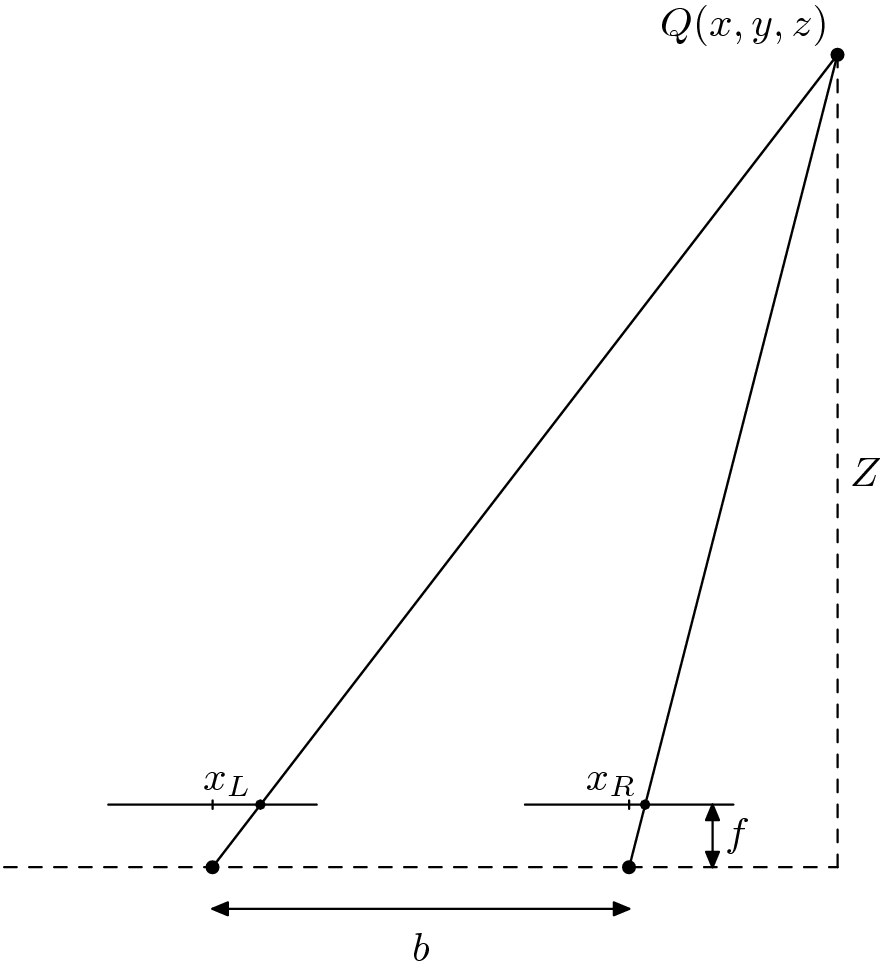
\includegraphics[width=9cm]{img/rekonstrukcija_udaljenosti.png}
  \caption{Skica uz rekonstrukciju udaljenosti}
  \label{fig:rekonstrukcija_udaljenosti}
\end{figure}

Slika predstavlja dvije kamere duž horizontalne iscrtkane linije, iznad kojih se
nalaze projekcijske ravnine. Trenutno promatramo točku u prostoru $Q(x, y, z)$ koja se projicira na navedene ravnine.
Projicirani pikseli se nalaze na apscisnim koordinatama $x_L$ lijeve slike i
$x_R$ desne slike uz pretpostavku da je ishodište u središtu ravnine projekcije. Udaljenost između kamera i promatrane točke označena je sa $Z$, žarišna
udaljenost s $f$, dok je razmak između kamera (eng. {\sl baseline}) označen s $b$.

Sada možemo izvesti izraz kojim ćemo dobiti udaljenost između kamere i promatrane točke prostora
koristeći navedene poznate parametre. Izvod se temelji na sličnosti trokuta. Iz trokuta lijeve kamere imamo
\begin{equation}
\frac{f}{x_L} = \frac{Z}{X} \label{lijevi_trokut}
\end{equation}
dok iz trokuta desne kamere imamo
\begin{equation}
\frac{f}{x_R} = \frac{Z}{X - b} \label{desni_trokut}
\end{equation}
Iz \ref{desni_trokut} možemo izvući $X$:
\begin{equation}
X = Z\frac{x_R}{f} + b \label{desni_x}
\end{equation}
i uvrštavanjem u \ref{lijevi_trokut} dolazimo do krajnjeg izraza
\begin{equation}
Z = \frac{fb}{d} \label{udaljenost}
\end{equation}
gdje je $d = x_L - x_R$ disparitet.
Sada možemo vidjeti da je udaljenost od kamere obrnuto proporcionalna disparitetu. To znači da što
je promatrani objekt bliže kameri, to će disparitet biti veći i obratno.

\chapter{Lokalne metode}
Metode guste stereoskopske rekonstrukcije se mogu podijeliti na lokalne i globalne. U ovom poglavlju ćemo načelno opisati takve metode te detaljnije obraditi neke koje su korištene u ovom radu.

Lokalne metode se temelje na principu prozorčića ili okna fiksne širine oko piksela. Označimo širinu prozora s $w$. Primijetimo kako bi $w$ trebao biti neparan broj jer se promatrani piksel
nalazi u sredini prozora, a sa svake strane oko njega nalazi se jednak broj piksela.

Ideja je da trčimo po svim pikselima lijeve slike te ih uspoređujemo s pikselima desne slike, ali
s određenim pomakom. Taj pomak naziva se disparitet i upravo je on cilj koji trebamo odrediti.
Kako je disparitet unaprijed zadan rasponom $[0, maksimalni\_disparitet]$, moramo se odlučiti
koji iz navedenog raspona ćemo odabrati. Naravno, odabrat ćemo onaj koji daje najbolje rezultate, no nekako moramo vrednovati takve rezultate. Rješenje leži u ideji da svakom mogućem
disparitetu dodijelimo cijenu koja opisuje u kakvom je odnosu piksel desne slike spram piksela
lijeve slike za koji želimo odrediti točan disparitet. Prirodno je da želimo proći što je
jeftinije moguće pa ćemo odabrati upravo onaj disparitet koji ima najmanju cijenu (eng. {\sl winner takes all}). Cijenu
također možemo shvatiti kao količinu razlike između intenziteta prozora oko odgovarajućih piksela.

Postavlja se pitanje što napraviti na rubovima slike gdje nije moguće izračunati sve vrijednosti prozora iz razloga što se koordinate piksela mogu nalaziti izvan slike. Nekoliko je mogućih rješenja:
\begin{itemize}
  \item računati samo piksele koje je moguće obuhvatiti unutar slike
  \item proširiti sliku crnim (intenziteta 0) okvirom širine $w/2$
  \item uopće ne računati korespondenciju za rub slike.
\end{itemize}

Svaki pristup ima svoje mane i prednosti. U vlastitoj implementaciji je korišteno treće rješenje gdje se uopće ne računa korespondencija na rubnim pikselima, radi jednostavnosti. Razlika u pogrešci je relativno
mala, a u skupu slika KITTI \footnote{http://www.cvlibs.net/datasets/kitti/eval\_scene\_flow.php?benchmark=stereo} su rubovi uglavnom i isključeni iz provjere točnih dispariteta.

Kod svake navedene metode korespondencije ćemo prikazati reultat na jednom paru slika (slike \ref{fig:lijeva_KITTI} i \ref{fig:desna_KITTI} iz skupa KITTI.

\begin{figure}[htb]
  \centering
  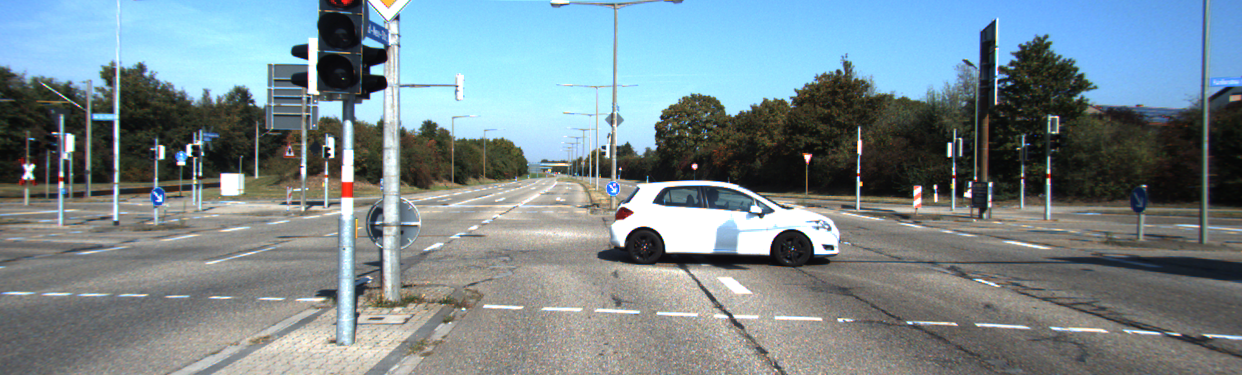
\includegraphics[width=14cm]{img/000046_10_2.png}
  \caption{Primjer slike iz lijeve kamere skupa KITTI}
  \label{fig:lijeva_KITTI}
\end{figure}

\begin{figure}[htb]
  \centering
  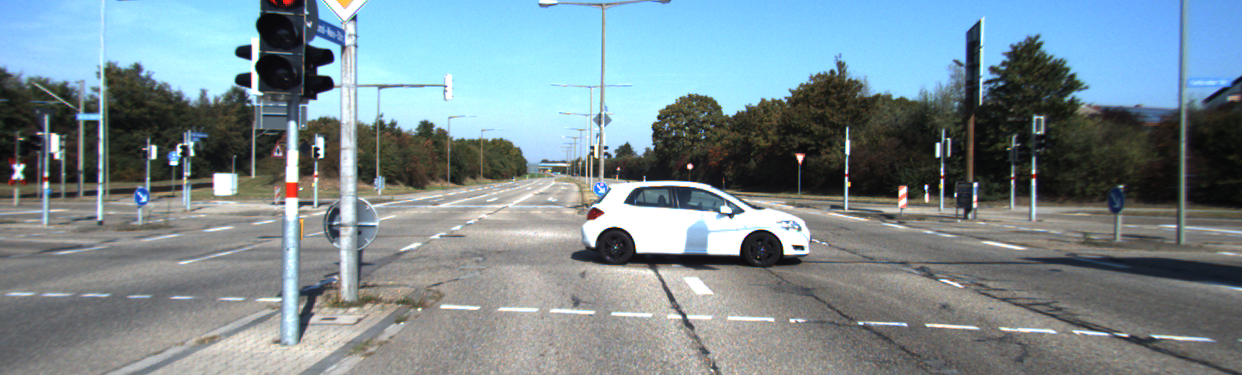
\includegraphics[width=14cm]{img/000046_10_3.png}
  \caption{Primjer slike iz desne kamere skupa KITTI}
  \label{fig:desna_KITTI}
\end{figure}

\section{Općeniti algoritam}
Sada ćemo opisati općeniti algoritam za lokalno podudaranje.

{\tt za svaki piksel $p(x, y)$ lijeve slike:}

{\quad \tt za svaki disparitet $0 \leq d \leq maksimalni\_ disparitet$:}

{\quad\quad\tt za svaki piksel $q(x', y')$ u prozoru piksela $p'(x - d, y)$ desne slike:}

{\quad\quad\quad \tt cijena[$y$][$x$] += $f(p, q)$}    


\noindent pri čemu je funkcija $f(x, y, d)$ funkcija korespondencije koja određuje cijenu razlike odgovarajućih piksela lijeve i desne slike. Svaki piksel lijeve slike s pozicijom $(x, y)$
uspoređuje se s pikselom desne slike u prozoru oko piksela na poziciji $(x - d, y)$, gdje je $d$ disparitet. Vidimo kako se odgovarajući pikseli nalaze na istoj $y$ koordinati što je posljedica rektifikacije slika.
Stoga je potrebno razmatrati samo piksele duž epipolarne linije.

\section{SSD}

Prva metoda koju ćemo opisati je SSD ({eng. \sl Sum of Squared Differences}) koja se temelji na zbroju kvadrata razlika intenziteta piksela.
Matematički ju možemo opisati sljedećim izrazom:
\[
C_{SSD}(x, y, d) = \sum(I_R(x - d, y) - I_L(x, y))^2
\]
gdje su $(x, y)$ koordinate piksela lijeve slike, $d$ trenutni disparitet, a $I_L$ lijeva slika te $I_R$ desna slika. Zbroj ide po svim pikselima unutar prozora promatranog piksela.
Najbolja podudarnost kod SSD-a postiže se kada je vrijednost funkcije cijene jednaka $0$. Lako je vidjeti zašto je tomu tako kada bismo usporedili dva prozora s istim intenzitetima piksela. Tada će vrijednost funkcije biti $0$ jer oduzimamo iste vrijednosti. Iz toga slijedi da što se intenziteti više razlikuju, to će i cijene biti veće. Također, kvadrat doprinosi tome da vrijednosti ne budu negativne tako da možemo raditi samo s pozitivnim brojevima.

\begin{figure}[htb]
  \centering
  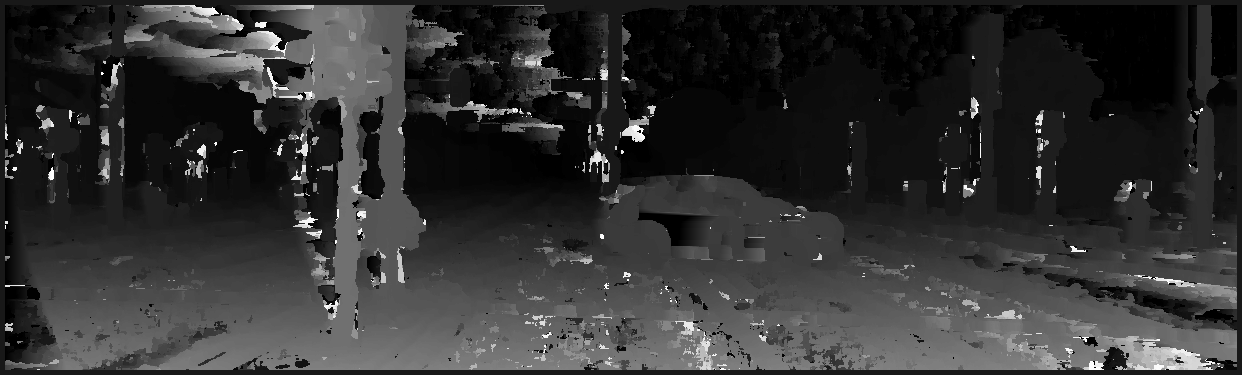
\includegraphics[width=14cm]{img/local_000046_10_SSD_11_140_scaled.png}
  \caption{Rezultat primjene metode SSD uz veličinu prozora 11}
  \label{fig:SSD-KITTI}
\end{figure}

\section{ZSAD}

Sljedeća metoda je ZSAD ({eng. \sl Zero Sum of Absolute Differences}). Matematički ju možemo definirati ovako:
\[
C_{ZSAD}(x, y, d) = \sum\lvert(M_L - I_L(x, y)) - (M_R - I_R(x - d, y))\rvert
\]
gdje je $I_L$ lijeva slika, $I_R$ desna slika, a $M_L$ i $M_R$ srednje vrijednosti intenziteta piksela u trenutnom prozoru lijeve, odnosno desne slike.
Nedostatak ove metode je što moramo računati i srednje vrijednosti svakog mogućeg prozora. Za razliku od SSD-a, ovdje nenegativnost cijena postižemo korištenje apsolutne vrijednosti, a ne kvadriranjem. Idealna vrijednost iznosi 0, odnosno u slučaju kada su svi odgovarajući pikseli u oba
prozora jednakih intenziteta.

\begin{figure}[htb]
  \centering
  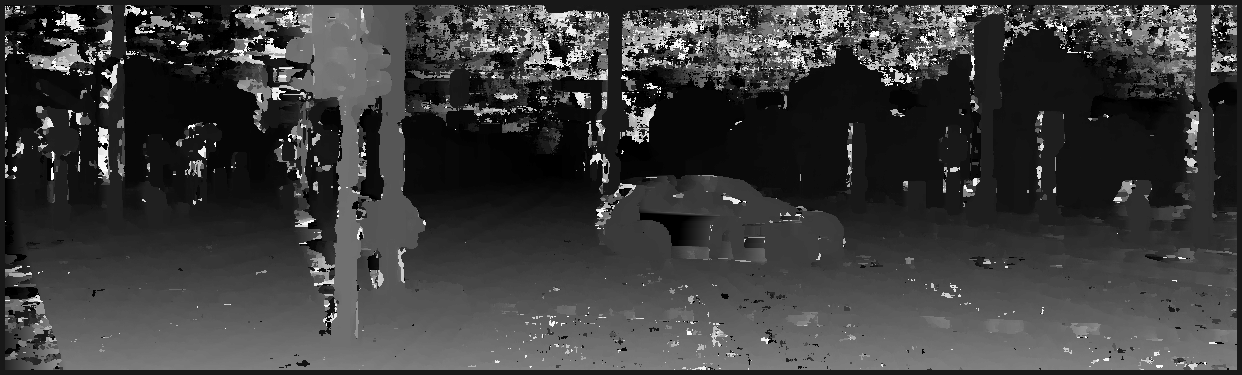
\includegraphics[width=14cm]{img/local_000046_10_ZSAD_11_140_scaled.png}
  \caption{Rezultat primjene metode ZSAD uz veličinu prozora 11}
  \label{fig:ZSAD-KITTI}
\end{figure}

\section{Census}

Funkcija korespondencije Census se temelji na Hammingovoj udaljenosti između dvije binarne riječi. Kako bismo odredili cijenu između dvaju piksela, potrebno je transformirati
prozore oko piksela u binarne riječi. Svakom pikselu u prozoru ćemo pridružiti bit prema sljedećoj funkciji:

\[   
b(p, q) = 
     \begin{cases}
       0, & I(p) \leq I(q) \\
       1, & I(p) > I(q) \\
     \end{cases}
\]
gdje je $I$ slika, $p$ piksel u sredini prozora za kojega računamo transformaciju, $q$ bilo koji piksel unutar prozora. Važno je napomenuti da redoslijed pridruživanja bitova mora biti jednak u oba
prozora koja se uspoređuju kako bi rezultat bio ispravan. Zgodno je primijetiti kako će
rezultat biti isti ukoliko zamijenimo vrijednosti gornjih jednadžbi, odnosno invertiramo bitove. Nakon što svakom pikselu pridružimo binarnu vrijednost, cijenu možemo izračunati
računski tako primijenimo operaciju isključivo-ili između binarnih riječi prozora lijeve i desne slike te zatim prebrojimo broj bitova u jedinici.

\begin{figure}[htb]
  \centering
  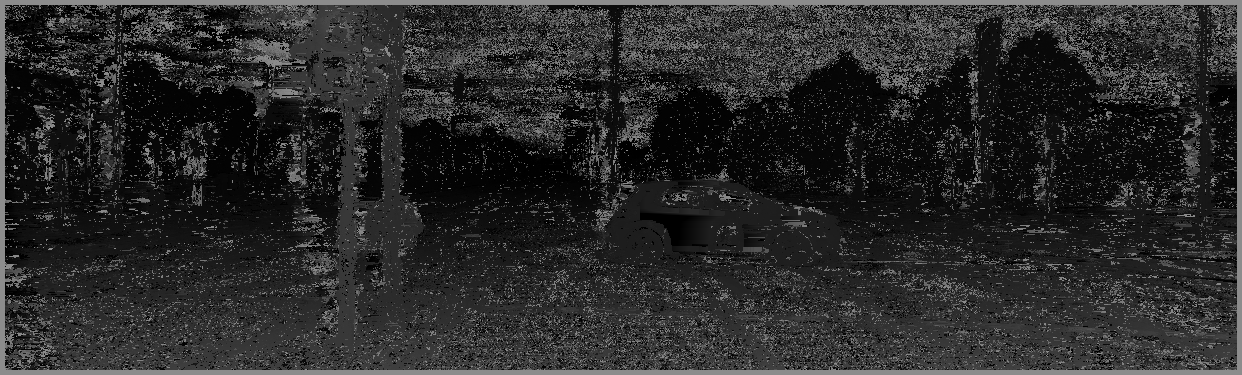
\includegraphics[width=14cm]{img/local_000046_10_Census_11_140.png}
  \caption{Rezultat primjene metode Census uz veličinu prozora 11}
  \label{fig:Census-KITTI}
\end{figure}

Do sada navedene metode opisane su u projektnoj dokumentaciji kolega \cite{projekt1415} te u članku \cite{hirschmuller2007evaluation}.

\section{Korespondencija neovisna o uzorkovanju}

Birchfield-Tomasijeva korespondencija se malo razlikuje od do sada navedenih metoda.
Razlikuje se po tome što ona ne koristi prozorčić već se temelji na usporedbama s dvaju susjednih piksela duž epipolarne linije.
Funkcija cijene je definirana preko simetričnih funkcija:
\[
C_{BT} = \min(C_{BT}(x_i, y_i, I_L, I_R), C_{BT}(y_i, x_i I_R, I_L)
\]
gdje se $x_i$ i $y_i$ pikseli lijeve slike $I_L$, odnosno desne slike $I_R$.

Funkcije $C_{BT}$ je definirana ovako:
\begin{equation}
I^+ = \frac{1}{2}(I_i(y_i) + I_R(y_i + 1))
\end{equation}

\begin{equation}
I^- = \frac{1}{2}(I_R(y_i) + I_R(y_i - 1))
\end{equation}

\begin{equation}
I_{min} = \min(I^-_R, I^+_R, I_R(y_i))
\end{equation}

\begin{equation}
I_{max} = \max(I^-_R, I^+_R, I_R(y_i))
\end{equation}

\begin{equation}
C_{BT}(x_i, y_i, I_L, I_R) = \max(0, I_L(x_i) - I_{max}, I_{min} - I_L(x_i)))
\end{equation}

\begin{figure}[htb]
  \centering
  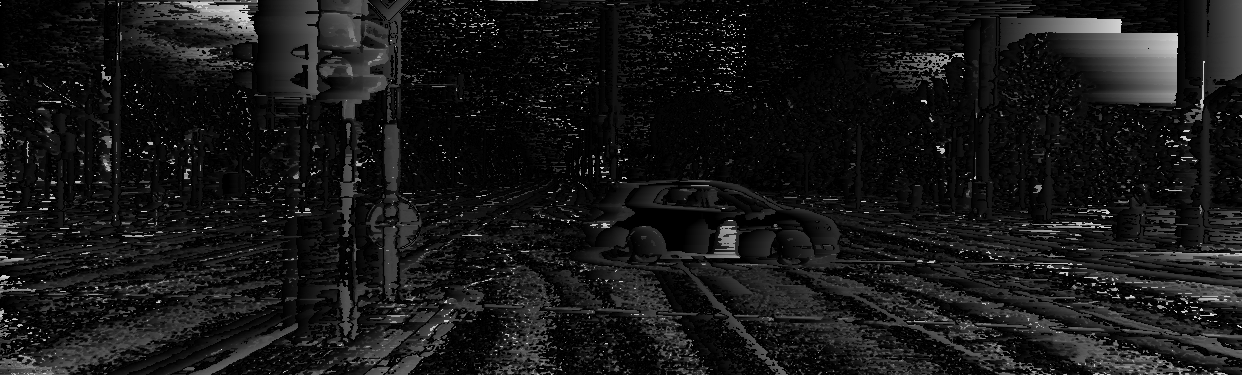
\includegraphics[width=14cm]{img/local_000046_10_BT_1_140_scaled.png}
  \caption{Rezultat primjene metode Birchfield-Tomasi}
  \label{fig:BT-KITTI}
\end{figure}

Birchfield-Tomasijeva cijena je opisana u diplomskom radu Dine Kovača \cite{kovac15ms}, a izvorno u radu Stana Birchfielda i Carla Tomasija \cite{birchfield1998depth}.

\section{Usporedba lokalnih i globalnih metoda}
U ovom odjeljku dana je usporedba lokalnih i globalnih metoda podudaranja.
U tablici se nalaze neka važnija svojstva lokalnih metoda s lijeve strane te
analognih svojstava globalnih metoda s desne strane.

\begin{table}[H]
  \caption{Svojstva lokalnih i globalnih metoda}
  \label{tbl:usp_lok_glob}
  \centering
  \begin{tabularx}{\textwidth}{X|X} \hline
    {\bf Lokalne metode} & {\bf Globalne metode} \\
    \hline
    cijene temeljene na prozorčićima oko svakog pojedinog piksela & cijene temeljene na svim pikselima slike \\
    \hline
    odabir pojedinog dispariteta po principu minimalne agregirane cijene & minimizacija globalne funkcije kroz vrijednosti svih piksela slike \\
    \hline
    značajno jednostavnije za implementaciju & teže za implementaciju \\
    \hline
    daju lošije rezultate & daju značajno bolje rezultate \\
    \hline
    u pravilu brže & u pravilu sporije \\
  \end{tabularx}
\end{table}

U sljedećem poglavlju ćemo uvesti algoritam poluglobalnog podudaranja koji kao ulaz prima cijene izračunate kod lokalne korespondencije, a optimizaciju radi nad svim
pikselima u određenim smjerovima. Time ga, kao što mu i naziv govori, možemo svrstati negdje između jer koristi lokalne korespondencije, a optimira (točnije, aproksimira) globalno.


\chapter{Poluglobalno podudaranje}

Sada ćemo oblikovati algoritam poluglobalnog podudaranja (eng. {\sl semi-global matching, SGM}).
Vidjeli smo kako funkcioniraju lokalne metode pa razmislimo koje nedostatke imaju. Jedan od nedostataka je što
smo kod traženja najsličnijeg piksela ograničeni veličinom prozorčića. Jedna loša strana je što ne možemo uzeti u obzir sve piksele, već moramo pogađati na temelju trenutnih spoznaja.
To ponekad dovodi do artefakata koji su dobro vidljivi na gornjim slikama, npr. slika \ref{fig:ZSAD-KITTI}.
Drugi nedostatak {\sl lokalnosti} je što dobivamo loše rezultate na rubovima glatkih površina
gdje dolazi do naglih prekida u dubini ili gdje ima čestih izmjena dubine.

Poluglobalno podudaranje pokušava otkloniti neke od navedenih nedostataka. Pokušajmo razmisliti kako bismo mogli unaprijediti postupak stereoskopske rekonstrukcije uz smanjenje navedenih nedostataka (ipak ih ne možemo u potpunosti izbjeći).

Prvo što bismo mogli napraviti jest ne promatrati samo malu konačnu okolinu piksela već proširiti područje traženja najboljeg dispariteta. Time bismo dobili bolju globalnu sliku jer se možemo bolje prilagoditi pretpostavci da radimo uglavnom s glatkim površinama.

Drugo poboljšanje koje bismo mogli uvesti je da na neki način forsiramo ograničenje glatkoće rekonstrukcije.
To možemo učiniti tako da za svaki disparitet probamo prvo uzeti okolne piksele s istim disparitetom, a svaku razliku u disparitetu kažnjavamo određenim povećanjem cijene.

Upravo navedena poboljšanja su glavne ideje algoritma poluglobalnog podudaranja. Algoritam se odvija u nekoliko koraka:
\begin{enumerate}
  \item izračun cijena korespondencija (pomoću ranije navedenih lokalnih metoda),
  \item agregacija cijena te
  \item odabir dispariteta s najboljim cijenama.
\end{enumerate}

Globalne metode obično definiraju globalnu funkcije energije koju pokušavaju optimirati.
No, taj postupak je izrazito zahtjevan pa poluglobalno podudaranje tome priskače na način
da aproksimira najbolju moguću energiju.

Definirajmo funkciju energije koja ovisi o disparitetu $D$ na sljedeći način:
\begin{equation} \label{energija}
E(D) = \sum_{\mathbf{p}}(C(\mathbf{p}, D_{\mathbf{p}}) + \sum_{\mathbf{q} \in N_{\mathbf{p}}} P_1 T [\lvert D_{\mathbf{p}} - D_{\mathbf{q}}\rvert = 1] + \sum_{\mathbf{q} \in N_{\mathbf{p}}} P_2 T [\lvert D_{\mathbf{p}} - D_{\mathbf{q}}\rvert > 1])
\end{equation}
gdje je $C(\mathbf{p}, D_{\mathbf{p}})$ cijena piksela $\mathbf{p}$ ovisno o pripadnom disparitetu, a $P_1$ i $P_2$ konstantni parametri koji predstavljaju kazne da diskontinuitete. Uvijek mora vrijediti $P_1 \leq P_2$.
Funkcija $T[x]$ je definirana na sljedeći način:
\[   
T[x] = 
     \begin{cases}
       0, & x\ \ je\ \ laž \\
       1, & x\ \ je\ \ istina \\
     \end{cases}
\]
Ideja je aproksimirati optimalnu vrijednost navedene funkcije energije, odnosno odabrati
mapu dispariteta $D$ za koju će vrijednost $E(D)$ biti minimalna.

Pretpostavimo da smo već izračunali cijene korespondencija koristeći neku od ranije navedenih lokalnih metoda.
Sljedeći korak je agregacija cijena. To ćemo provesti tako da za svaki piksel računamo cijene
po putevima u različitim smjerovima. Preporučeno je da bude barem 8, a idealno bi bilo 16 puteva. Ti putevi su ilustrirani na slici \ref{fig:SGM} (16 puteva). Cijena po putu $\mathbf{r}$
može se opisati sljedećom rekurzivnom funkcijom:
\begin{equation} \label{cijena_1}
  \begin{split}
    L'_{\mathbf{r}}(\mathbf{p}, d) = & C(\mathbf{p}, d) + \min(L'_{\mathbf{r}}(\mathbf{p} - \mathbf{r}, d), \\
    & L'_{\mathbf{r}}(\mathbf{p} - \mathbf{r}, d - 1) + P_1, \\
    & L'_{\mathbf{r}}(\mathbf{p} - \mathbf{r}, d + 1) + P_1, \\
    & \min\limits_{i} L'_{\mathbf{r}}(\mathbf{p} - \mathbf{r}, i) + P_2) \\
  \end{split}
\end{equation}
gdje je $\mathbf{p}$ trenutni piksel, $d$ trenutni disparitet, $C(\mathbf{p}, d)$ ranije
izračunata cijena, a $P_1 \leq P_2$ fiksni, unaprijed određeni parametri koji kažnjavaju
prekide u kontinuitetu.

Probajmo sada riječima opisati što funkcija radi. Za trenutni piksel agregira unaprijed izračunatu cijenu te joj pridodaje minimalnu cijenu puta prošlog piksela ovisno o najboljem disparitetu. Vidimo da se u ovom koraku događa spomenuto kažnjavanje.
Ukoliko se disparitet razlikuje malo (u ovom slučaju točno 1), tada ćemo dodati malu kaznu $P_1$ na cijenu, a ukoliko
se razlikuje puno (u ovom slučaju više od 1), onda ćemo dodati veću kaznu $P_2$.

\begin{figure}[H]
  \centering
  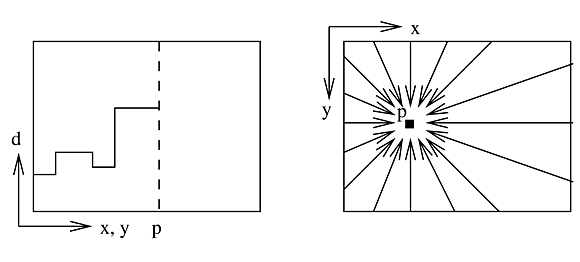
\includegraphics[width=12cm]{img/sgm.png}
  \caption{Ilustracija rada algoritma poluglobalnog podudaranja}
  \label{fig:SGM}
\end{figure}


Primijetimo sada jedan nedostatak ove funkcije. Kako agregiramo cijene duž određenog puta, cijena puta uvijek raste i može poprimiti veliku vrijednost. Tome ćemo doskočiti tako da od trenutne cijene puta oduzmemo najmanju cijenu puta u prošlom koraku, što je opisano u \ref{cijena_puta}.
Ova modifikacija neće promijeniti put jer je ta vrijednost konstantna za sve disparitete konkretnog piksela. Stoga se disparitet s najmanjom cijenom, tj. minimum funkcije, neće promijeniti.
Najveća vrijednost cijene će sada biti $L \leq C_{\max} + P_2$.

\begin{equation} \label{cijena_puta}
  \begin{split}
    L_{\mathbf{r}}(\mathbf{p}, d) = & C(\mathbf{p}, d) + \min(L_{\mathbf{r}}(\mathbf{p} - \mathbf{r}, d), \\
    & L_{\mathbf{r}}(\mathbf{p} - \mathbf{r}, d - 1) + P_1, \\
    & L_{\mathbf{r}}(\mathbf{p} - \mathbf{r}, d + 1) + P_1, \\
    & \min\limits_{i} L_{\mathbf{r}}(\mathbf{p} - \mathbf{r}, i) + P_2) - \min\limits_{k}L_{\mathbf{r}}(\mathbf{p} - \mathbf{r}, k) \\
  \end{split}
\end{equation}

Agregiranje cijena provodimo po svim putevima $\mathbf{r}$. Kako bi se dobio zadovoljavajući rezultat,
preporučeno je barem 8 puteva kako bi se što bolje pokrila cijela slika. U slučaju 8 puteva, jasno je kako se treba kretati (po horizontalnim i vertikalnim osima te po dijagonalama), no što u slučaju 16 smjerova?
Tada se još treba kretati i između dijagonala, a to ćemo postići tako da se pomaknemo 2 piksela horizontalno, a zatim 1 vertikalno ili obratno što je prikazano na slici \ref{fig:SGM-paths}. Pretpostavljamo da je ishodište koordinatnog sustava slike u gornjem lijevom kutu, pozitivni smjer apscise je udesno, a ordinate prema dolje.

Nakon što smo izračunali cijene za sve puteve, sada cijenu pojedinog dispariteta za određeni
piksel možemo izraziti sljedećom funkcijom:
\begin{equation}
  S(\mathbf{p}, d) = \sum_{\mathbf{r}}L_{\mathbf{r}}(\mathbf{p}, d)
\end{equation}
čija najveća vrijednost će biti 16 puta već od najveće cijene pojedinog puta iz razloga što
ćemo svaki piksel obići 16 puta (ukoliko radimo sa 16 smjerova). Dakle, vrijedi $S \leq 16(C_{\max} + P_2)$.

Označimo širinu slike s $W$, visinu s $H$, a najveći disparitet s $D$.
Postupak računanja radimo tako da krenemo od rubnih piksela slike i računamo po \ref{cijena_puta}. Za to nam je potrebno polje $S[W][H][D]$ (početno inicijalizirano na 0) u koje ćemo pohranjivati izračunate cijene.


\begin{figure}[H]
  \centering
  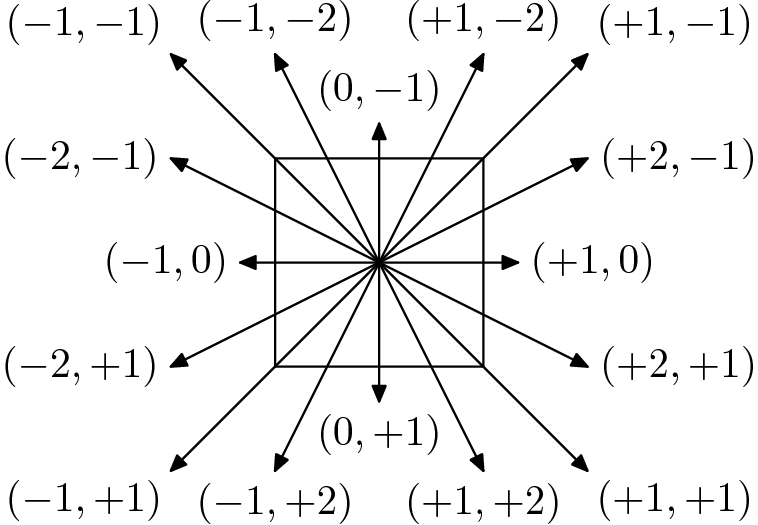
\includegraphics[width=10cm]{img/sgm_smjerovi.png}
  \caption{Ilustracija smjerova kretanja kod agregacije cijena}
  \label{fig:SGM-paths}
\end{figure}

Sljedeći korak nakon agregacije je odabrati najbolju mapu dispariteta, a to radimo na identičan način
kao kod lokalnih metoda---odabirom dispariteta s najmanjom cijenom.

Pokušajmo sada odrediti kolika je složenost navedenog postupka. Pretpostavimo da radimo sa 16 smjerova. Kako krećemo od svakog rubnog piksela i širimo se u svim mogućim smjerovima, svaki
piksel ćemo posjetiti 16 puta, iz svakog smjera jedanput, i tako za svaki mogući disparitet. Iz toga slijedi da je složenost postupka $O(16WHD)$, tj. $O(WHD)$.
Minimalnu cijenu puta prošlog piksela možemo izračunati u složenosti $O(D)$, ali pošto je konstantna za sve disparitete trenutnog piksela, možemo ju unaprijed izračunati. Zaključujemo da je složenost algoritma vrlo povoljna (linearna), pogotovo u kombinaciji sa korespondencijom Birchfield-Tomasi.

Također, zbog svoje pravilne strukture, algoritam je pogodan za korištenje vektorskih instrukcija. Najveći nedostatak je memorijska zahtjevnost. Autor algoritma kao rješenje tog problema predlaže
razlaganje velike slike na više manjih segmenata koji se preklapaju, te zatim provođenje algoritma kako je opisano, za svaki segment posebno.

Algoritam poluglobalnog podudaranja izvorno je opisao Heiko~Hirschm{\"u}ller \cite{hirschmuller2008stereo}, a alternativno objašnjenje je proučeno iz diplomskog rada Dine Kovača \cite{kovac15ms}.

\chapter{Opis implementacije}

Navedeni algoritmi implementirani su u programskom jeziku C++, a ispitni slijedovi, kao i pomoćne skripte napisani su u programskom jeziku Python verzije 3.
Operacijski sustav na kojemu je implementacija razvijana i isprobana jest GNU/Linux distribucija Debian.
Kako biste mogli pokrenuti programe, prvo je potrebno prevesti izvorni kod. Za to je potrebno imati kompajler, preporučeno g++, verzije koja podržava barem standard C++11.
Potrebno je imati sljedeće:
\begin{itemize}
\item C++ kompajler (isprobano na g++ verzije 6.3.0 \footnote{https://gcc.gnu.org/})
\item biblioteka png++, C++ omotač oko izvorne PNG biblioteke \footnote{http://www.nongnu.org/pngpp/}
\item OpenMP biblioteka \footnote{http://www.openmp.org/}
\item Python (isprobano u Pythonu 3)
\item biblioteka matplotlib (Python) za izradu grafova
\end{itemize}

Osim navedenoga, potrebno je preuzeti i raspakirati standardne skupove slika Middlebury i
KITTI.

Prvo ćemo krenuti s prevođenjem programa. U direktoriju s k\^odom nalazi se nekoliko Bash skripti koje olakšavaju prevođenje programa. Prva skripta koju trebate pokrenuti je
\begin{verbatim}
          ./compileStereoMatching.sh
\end{verbatim}
Ona prevodi sve potrebne lokalne metode korespondencije kao i implementacije lokalnog podudaranja te poluglobalnog podudaranja. Prevedeni program omogućava obradu jednog para slika (s lijeve i desne kamere) uz određene parametre te pohranjuje dobivene neskalirane mape dispariteta
u obliku PNG (eng. {\sl Portable Network Graphics}) slika. Naredba za pokretanje je sljedeća:
\begin{verbatim}
./stereoMatching lijeva_slika desna_slika metoda_korespondencije\
 velicina_prozora maksimalni_disparitet P1 P2 izlaz_lokalno izlaz_SGM
\end{verbatim}
Metoda korespondencije može biti SSD, ZSAD, Census ili BT. $P_1$ i $P_2$ su parametri kažnjavanja
diskontinuiteta kod algoritma poluglobalnog podudaranja. Kao što vidimo, program obrađuje slike
i lokalnim i poluglobalnim podudaranjem odjednom, koristeći istu metodu korespondencije.
Važno je naglasiti kako veličina prozora mora biti neparan broj jer se piksel oko kojega se računa cijena nalazi u sredini prozora pa sa svake strane mora biti jednak broj piksela.
Nepoštivanje navedenog ograničenja rezultirat će upozorenjem.

Drugi program za obradu slika omogućava korištenje poluglobalnog podudaranja i metode korespondencije Birchfield-Tomasi, što je kombinacija koja daje najbolje rezultate uz odličnu brzinu.
Njega možete prevesti naredbom:
\begin{verbatim}
          ./compileSGM.sh
\end{verbatim}

Izvođenje skripte rezultirat će izvršnim programom {\tt sgm}. Njega možete pokrenuti sljedećom naredbom:
\begin{verbatim}
     ./sgm lijeva_slika desna_slika maksimalni_disparitet P1 P2 izlaz
\end{verbatim}
gdje su $P_1$ i $P_2$ ponovo iznosi penala diskontinuiteta kod poluglobalnog podudaranja.
Pokretanje navedenog programa rezultirat će jednom neskaliranom mapom dispariteta pohranjenom
u obliku slike u formatu PNG.
Podrazumijevani broj smjerova optimizacija kod algoritma SGM je 16. Ukoliko se želi promijeniti
broj smjerova, potrebno je promijeniti varijablu {\verb|N_PATHS|} u npr. 8, te ponovo prevesti izvorni kod. Mape dispariteta su pohranjene u sivoj skali (eng. {\sl grayscale}).
Važno je pripaziti na to da mora vrijediti $P_1 \leq P_2$\/!

Osim programa za obradu slika stereoskopskom rekonstrukcijom, tu su još i dva pomoćna programa. Jedan omogućava skaliranje vrijednosti svih piksela slike u formatu PNG. Možete ga prevesti
naredbom
\begin{verbatim}
          ./compileScaler.sh
\end{verbatim}
što će rezultirati jednim izvršnim programom naziva {\tt scaleImage}. Pokretanje programa
izgleda ovako:
\begin{verbatim}
          ./scaleImage slika faktor_skaliranja nova_slika
\end{verbatim}
gdje je faktor skaliranja broj koji određuje koliko puta će se intenzitet svakog piksela povećati. Pretpostavlja se da se radi s pikselima u sivoj skali. Razlog implementiranja ovog programa
je što su kod manjih slika mape dispariteta skalirane kako bi se bolje vidjele razlike u dubini slike. Ako ne bi bilo skaliranja, slika bi bila previše tamna. Primjerice, kod standardnog skupa Middlebury je potrebno skalirati slike ukoliko se ne radi sa slikama u izvornoj rezoluciji. Razlog tome je jasan, ukoliko je slika manja, i najveći mogući disparitet će biti manji.
Time će i mapa dispariteta sadržavati manje vrijednosti intenziteta piksela.

Drugi pomoćni program je evaluator pojedine mape dispariteta. Moguće ga je prevesti naredbom:
\begin{verbatim}
          ./compileEvaluator.sh
\end{verbatim}
nakon čega će se u direktoriju stvoriti program {\tt evaluator}. Evaluator služi za ispitivanje
pogreške mape dispariteta pripadnog para slika u odnosu na temeljnu istinu (eng. {\sl ground truth}). Temeljna istina, ili mapa točnih dispariteta je dana u standardnim skupovima slika, 
obično u podskupu za treniranje. Program pokrećemo na sljedeći način:
\begin{verbatim}
     ./evaluator lijevi_tocni_disp desni_tocni_disp mapa_dispariteta
\end{verbatim}
što će rezultirati ispisom pogreške u konzoli. Pogreška je u rasponu $[0, 1]$ te ju možemo lako pretvoriti u postotke množenjem sa 100. Podrazumijevanja tolerancija između uspoređivanih vrijednosti je 3. Razlog primanja dvije slike je taj što su neki
pikseli zaklonjeni, odnosno vidi ih se samo iz jedne kamere te na zajedničkoj mapi dispariteta
zapravo ne znamo koja vrijednost bi tu trebala biti. Zato u obzir uzimamo samo piksele koji se vide na obje slike.
Također, obično su nepoznati dispariteti označeni crnom bojom (vrijednost 0 u sivoj skali), što evaluator uzima u obzir.

Osim navedenih programa, napisano je i nekoliko skripti u Pythonu. Prva koju ćemo opisati je
{\verb|middlebury_2006.py|} koja služi za ispitivanje navedenog standardnog skupa slika.
Pokrećemo ju naredbom:
\begin{verbatim}
          python3 middlebury_2006.py put_do_skupa_middlebury
\end{verbatim}
što će rezultirati stvaranjem direktorija {\verb|middlebury_2006_results|} u kojemu će se, nakon
obrade slika, nalaziti izračunate mape dispariteta. Slike se obrađuju pomoću ranije navedenog
programa {\verb|stereoMatching|}, i to pomoću svih implementiranih lokalnih metoda korespondencije, lokalnim
podudaranjem te poluglobalnim podudaranjem u zadanom rasponu veličina prozorčića.
Nakon što obrada slika završi, moguće je, po potrebi skalirati vrijednosti intenziteta
pozivanjem
\begin{verbatim}
          python3 scale.py direktorij_s_rezultatima faktor_skaliranja
\end{verbatim}

Nakon toga je sve spremno za generiranje grafova. Izvršavanjem naredbe
\begin{verbatim}
          python3 middlebury_plot.py
\end{verbatim}
dobit ćemo prikaz svih grafova pogrešaka korespondencija, zatim korespondencija u kombinaciji
s poluglobalnim podudaranjem te naposlijetku prikaz prosječnih pogrešaka u ovisnosti o
veličini prozorčića.

Za skup KITTI je napisana skripta {\verb|kitti_2015_sgm.py|} koja računa mape dispariteta
na skupu KITTI 2015 i to koristeći poluglobalno podudaranje u kombinaciji s Birchfield-Tomasijevom korespondencijom. Nakon pokretanja naredbe
\begin{verbatim}
          python3 kitti_2015_sgm.py put_do_skupa_kitti_2015
\end{verbatim}
nastat će direktorij {\verb|kitti_2015_sgmbt_results|} u kojem će se nalaziti izračunate
mape dispariteta za sve slike iz skupa za treniranje, iz razloga što samo za njih imamo točne
disparitete za usporedbu.

Nakon obrade, slike možemo evaluirati pozivom
\begin{verbatim}
          python3 kitti_2015_results.py put_do_skupa_kitti_2015
\end{verbatim}
te ćemo u konzoli dobiti ispis slike s najmanjom pogreškom, slike s najvećom pogreškom te
prosječnom pogreškom na cijelom skupu.



\chapter{Rezultati}

Implementirani algoritmi evaluirani su na standardnim skupovima slika Middlebury i KITTI.
Prvi dio evaluacije odrađen je na skupu Middlebury i cilj je bio usporediti s jedne strane lokalne metode
uz uzimanje dispariteta s najmanjom cijenom, a s druge strane lokalne metode u kombinaciji s
algoritmom poluglobalnog podudaranja. Posebno su izdvojene pogreške poluglobalnog podudaranja
u kombinaciji s BT cijenom. Parametri kažnjavanja bili su postavljeni na $P_1 = 3$ i $P_2 = 22$.
Na skupu KITTI je cilj bio vidjeti točnost algoritma poluglobalnog podudaranja u kombinaciji
s BT cijenom, i to s 8 i 16 smjerova, radi usporedbe tog parametra. Pokazat ćemo za svaku
varijantu slike s najmanjom i najvećom pogreškom te prosječnu pogrešku. Prvo ćemo krenuti sa skupom Middlebury.

\section{Middlebury}

Očekujemo kako će lokalne metode dati relativno dobre rezultate te da će uz uključivanje
SGM-a pogreška dodatno pasti. Vidjet ćemo kako će se ponašati SGM te u kojim segmentima će
dati poboljšanja i kolika, a u kojima neće biti velikih promjena.

Na prva dva grafa možemo vidjeti pogreške dobivene korištenjem metode korespondencije SSD, te
SSD uz kombinaciju sa SGM-om. SSD nudi relativno dobre rezultate, ali postoje i bolje
metode. Kada u igru uključimo SGM, vidimo da su se točnosti popravile pri jako malim
prozorima. 

\begin{figure}[H]
  \centering
  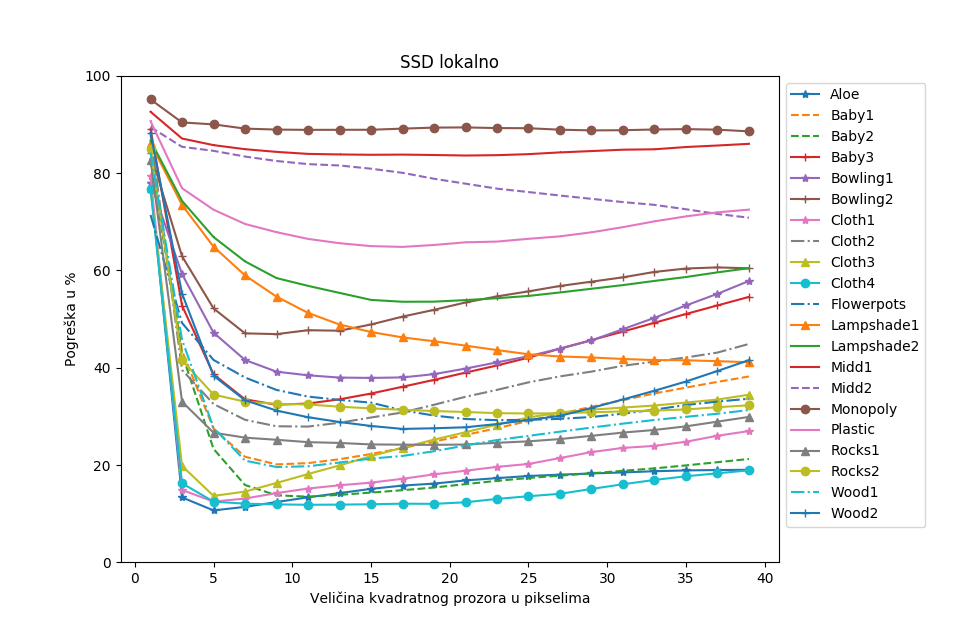
\includegraphics[width=13cm]{img/SSD_lokalno_middlebury.png}
  \caption{Pogreška metode korespondencije SSD}
  \label{fig:SSD-error}
\end{figure}

\begin{figure}[H]
  \centering
  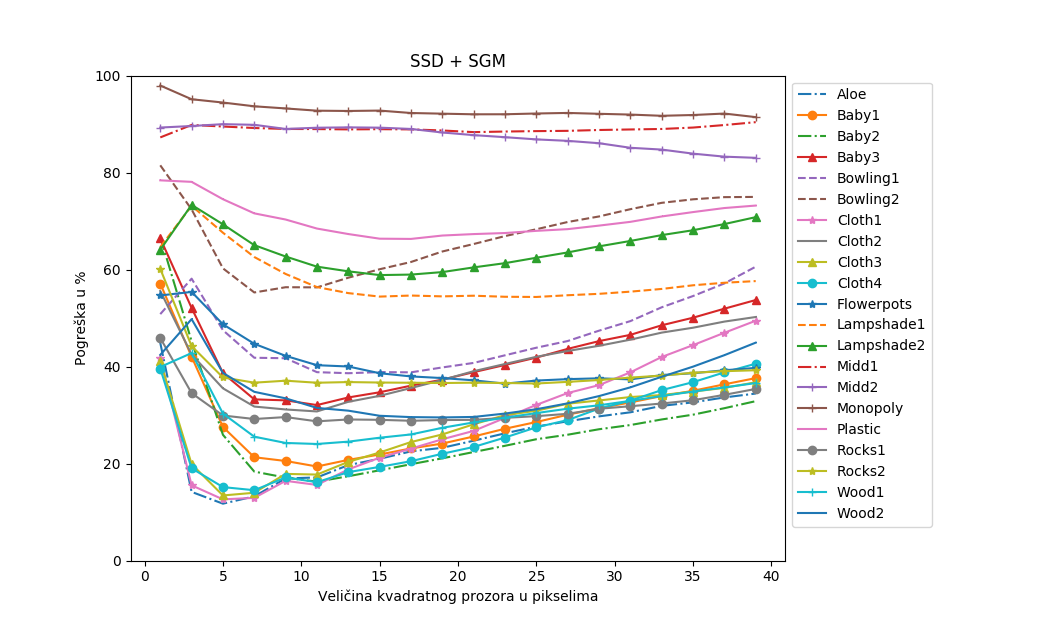
\includegraphics[width=13cm]{img/SSD_sgm_middlebury.png}
  \caption{Pogreška metode korespondencije SSD + SGM}
  \label{fig:SSD-sgm-error}
\end{figure}

Metoda ZSAD se pokazala kao najbolja u čisto lokalnoj varijanti. Vidimo da je
za većinu slika pogreška oko 20\%, i to za prozor veličine 5. Interesantno je da
uz kombinaciju sa SGM-om postiže još bolje rezultate, i to za prozor manji od
najboljeg u čisto lokalnoj varijanti.

\begin{figure}[H]
  \centering
  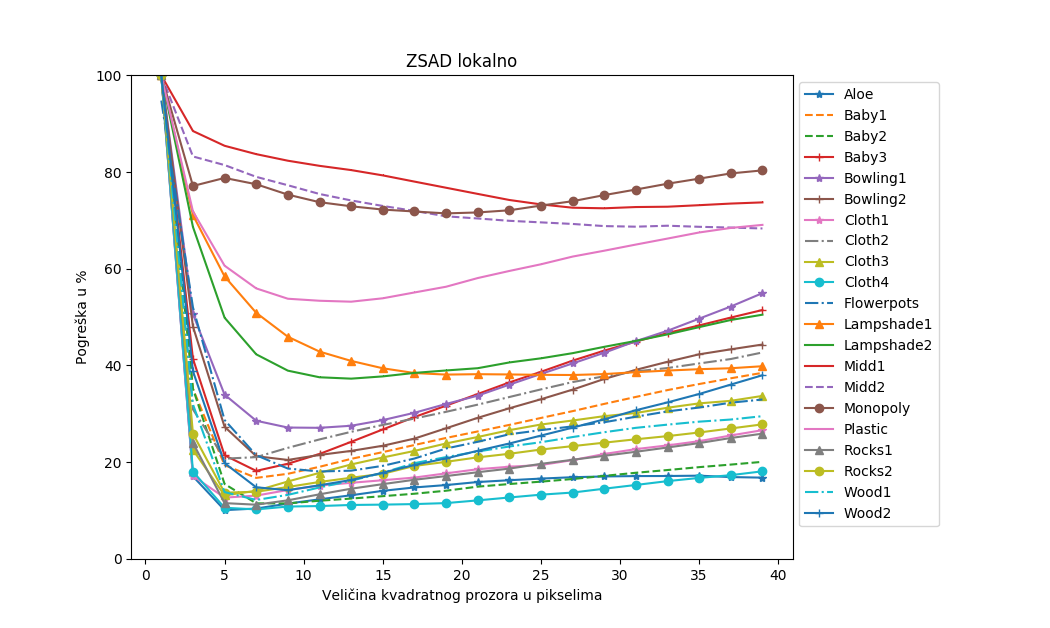
\includegraphics[width=13cm]{img/ZSAD_lokalno_middlebury.png}
  \caption{Pogreška metode korespondencije ZSAD}
  \label{fig:ZSAD-error}
\end{figure}

\begin{figure}[H]
  \centering
  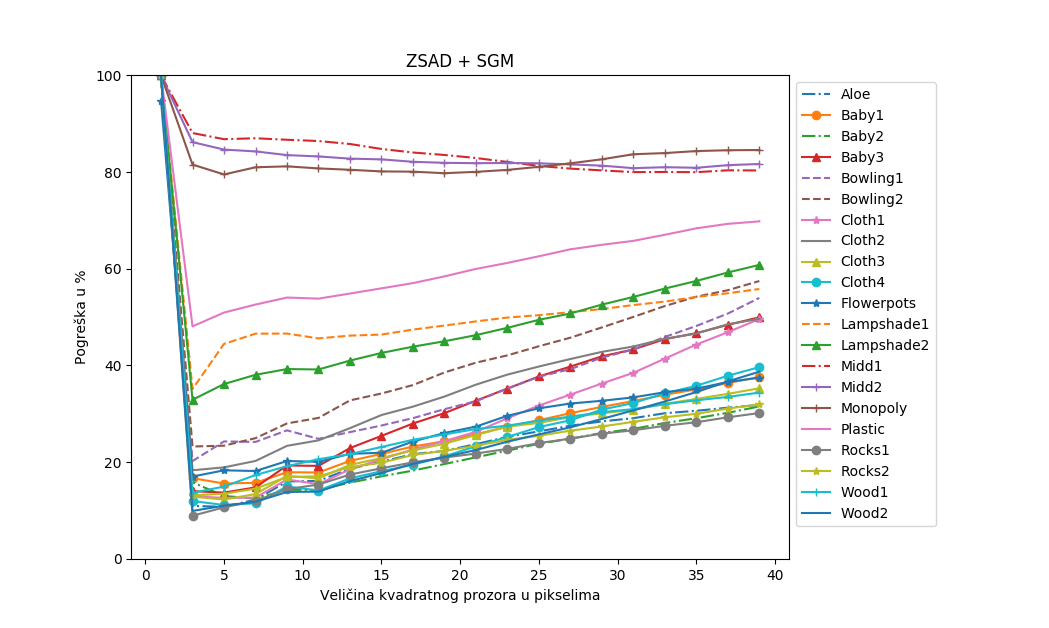
\includegraphics[width=13cm]{img/ZSAD_sgm_middlebury.png}
  \caption{Pogreška metode korespondencije ZSAD + SGM}
  \label{fig:ZSAD-sgm-error}
\end{figure}

Metoda Census je uvjerljivo najlošija u čisto lokalnoj varijanti, ali je iznenađujuće dobra
u kombinaciji sa SGM-om. To možemo objasniti ako pogledamo sliku \ref{fig:Census-KITTI}.
Vidimo da ima puno šuma, tj. pojedinih piksela koji odskaču od okoline. SGM-u ``odgovara''
takvo ponašanje jer je on dobar u ispravljanju manjih diskontinuiteta u zamjenu za glatkije
površine. Isto vrijedi i za metode SSD i ZSAD, kod korištenja manjih prozora. U ovom
slučaju Census i SGM daju bolje od rezultate od ZSAD-a u kombinaciji sa SGM-om.

\begin{figure}[H]
  \centering
  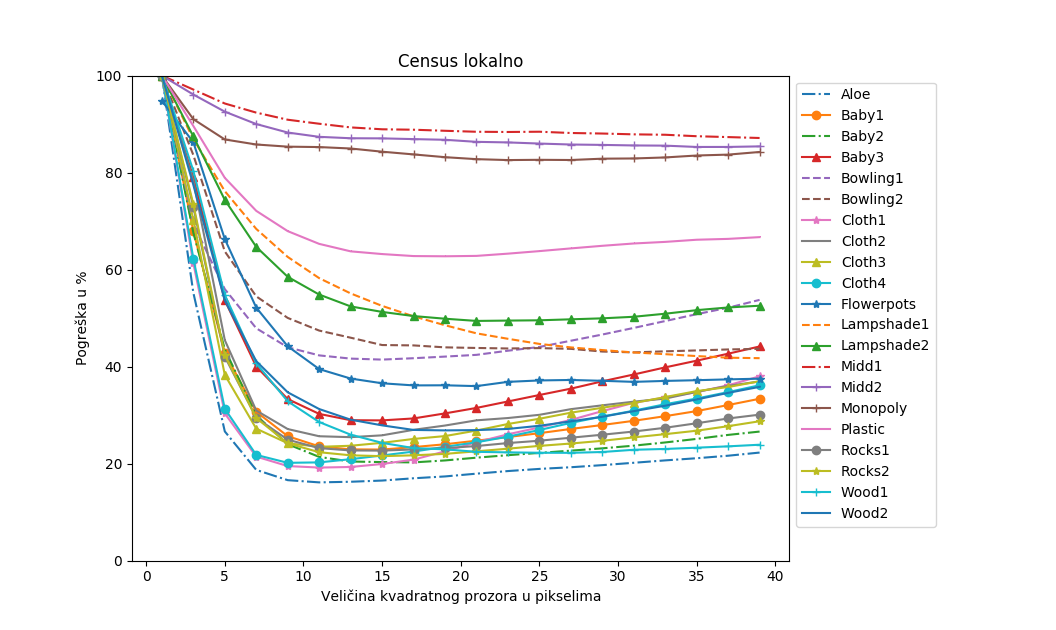
\includegraphics[width=13cm]{img/Census_lokalno_middlebury.png}
  \caption{Pogreška metode korespondencije Census}
  \label{fig:Census-error}
\end{figure}

\begin{figure}[H]
  \centering
  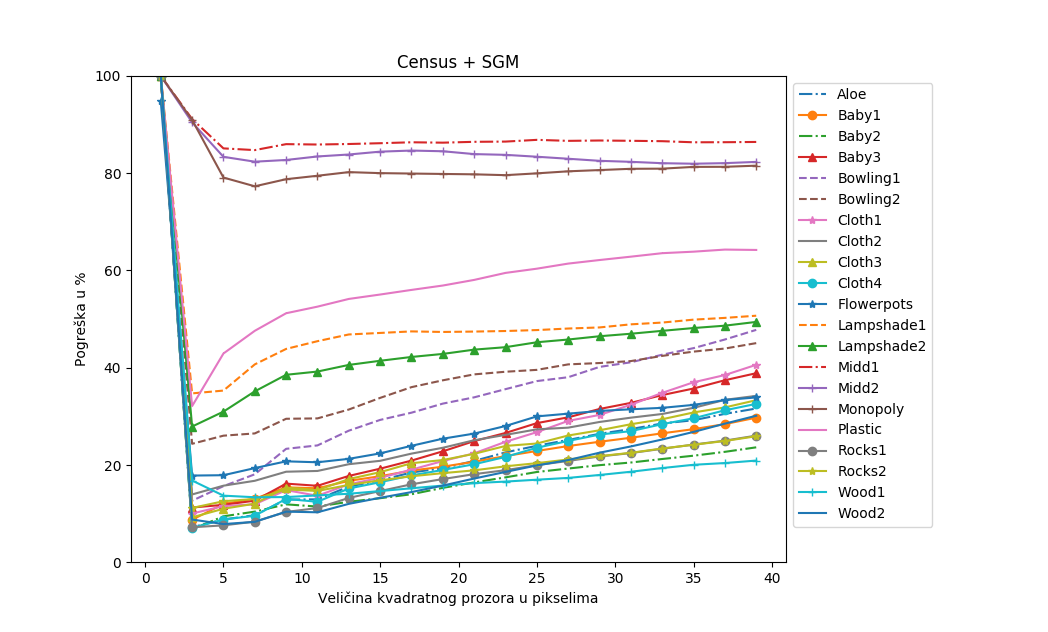
\includegraphics[width=13cm]{img/Census_sgm_middlebury.png}
  \caption{Pogreška metode korespondencije Census + SGM}
  \label{fig:Census-sgm-error}
\end{figure}

Na slikama \ref{fig:pogreska-lok} i \ref{fig:pogreska-sgm} možemo vidjeti prosječne vrijednosti pogreške metoda SSD, ZSAD i Census na
slici (a) te istih metoda u kombinaciji sa SGM-om na slici (b). To nam potvrđuje kako ZSAD
daje najbolje rezultate u samostalnoj varijanti, a Census u kombinaciji sa SGM-om.
Također vidimo da kako veličina prozora raste, SGM ima sve manje utjecaja, što je već objašnjeno
njegovim favoriziranjem šuma. Kod velikih prozora nema puno šuma, tj. sve površine su dosta velike i glatke te SGM zapravo nema što popravljati. Na slici \ref{fig:bt-sgm-error} još su
prikazane pogreške dobivene SGM-om u izvornoj varijanti, uz korespondenciju Birchfield-Tomasi.

\begin{figure}[H]
  \centering
  \subfloat[Pogreška lokalnih metoda]{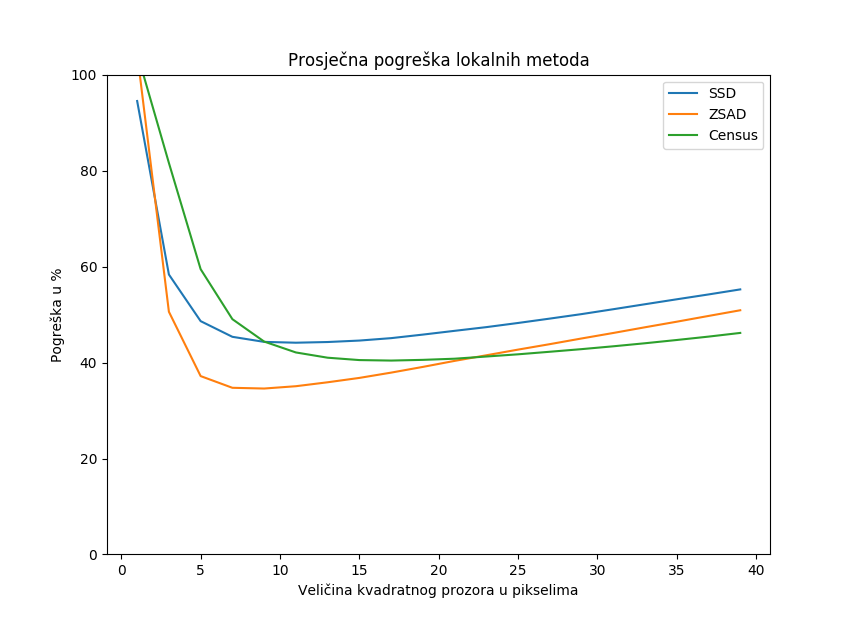
\includegraphics[width=0.5\textwidth]{img/prosjek_lokalno.png}\label{fig:pogreska-lok}}
  \hfill
  \subfloat[Pogreška lokalno + SGM]{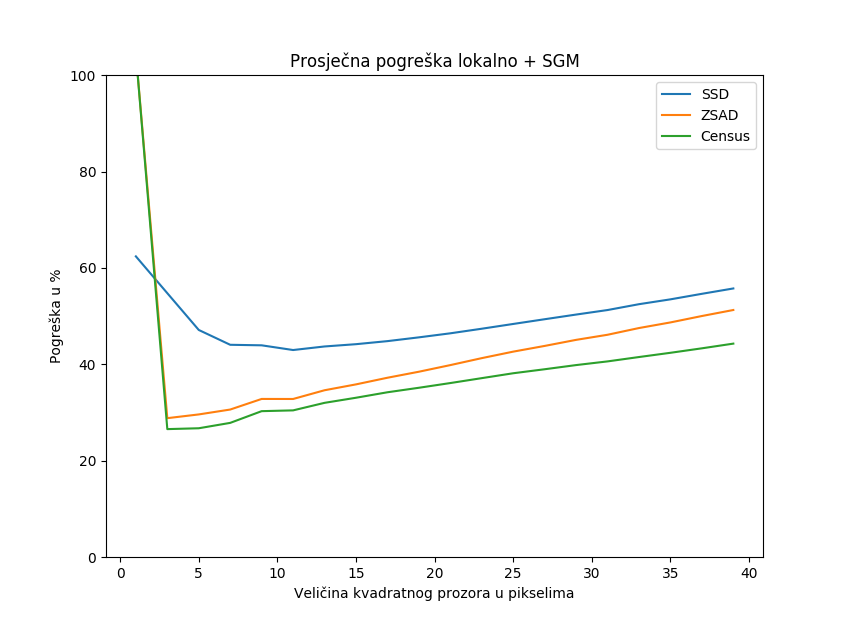
\includegraphics[width=0.5\textwidth]{img/prosjek_sgm.png}\label{fig:pogreska-sgm}}
  \caption{Prosječne pogreške u ovisnosti o veličini prozora}
\end{figure}

\begin{figure}[H]
  \centering
  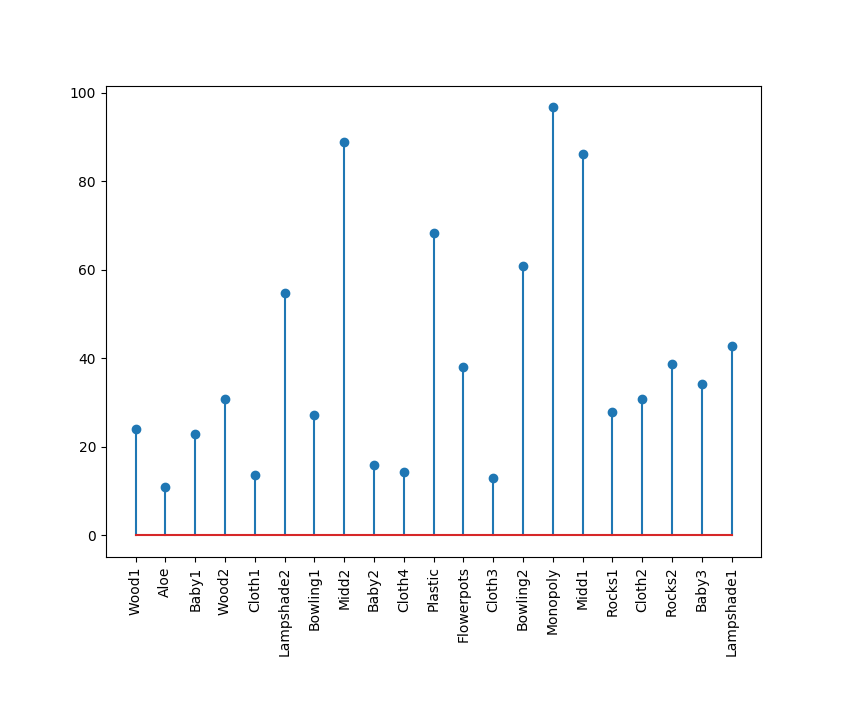
\includegraphics[width=13cm]{img/sgm_bt_middlebury.png}
  \caption{Pogreška metode korespondencije BT + SGM}
  \label{fig:bt-sgm-error}
\end{figure}

\section{KITTI}
Na skupu KITTI testiran je SGM u varijanti s 8 i 16 smjerova agregiranja cijena.
Testiranje je provedeno na skupu za treniranje uz koji su dane i mape točnih dispariteta
kako bi se mogle usporediti s izračunatima. Radi jednostavnosti, prikazivat ćemo samo slike
lijeve kamere.

Prvo ćemo pokazati sliku s najmanjom pogreškom, tj. najbolji rezultat. Slika iz skupa koja je imala najmanju
pogrešku je {\verb|000188_10.png|} i prikazana je na slici \ref{fig:kitti-min-sgm-error}.
Ista slika je imala najmanju pogrešku u obje varijante algoritma. Vidimo da slika predstavlja
relativno glatke i široke površine što je pogodno za SGM. Mogli bismo pretpostaviti da rezultat neće biti tako dobar
zbog šume s lijeve strane ceste, no kao što možemo vidjeti na mapi točnih dispariteta, taj dio
se ne uzima u obzir, niti je vidljiv na izračunatoj mapi dispariteta.

\begin{figure}[H]
  \centering
  \subfloat[Slika s najmanjom pogreškom u skupu KITTI]{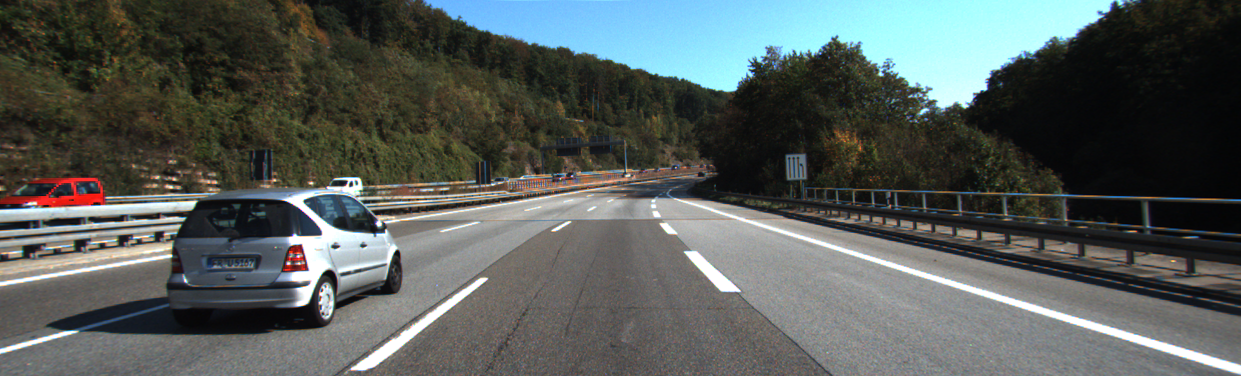
\includegraphics[width=13cm]{img/sgm_best_kitti.png}\label{fig:kitti-min-sgm-error}}
  
  \centering
  \subfloat[Pripadni točni dispariteti]{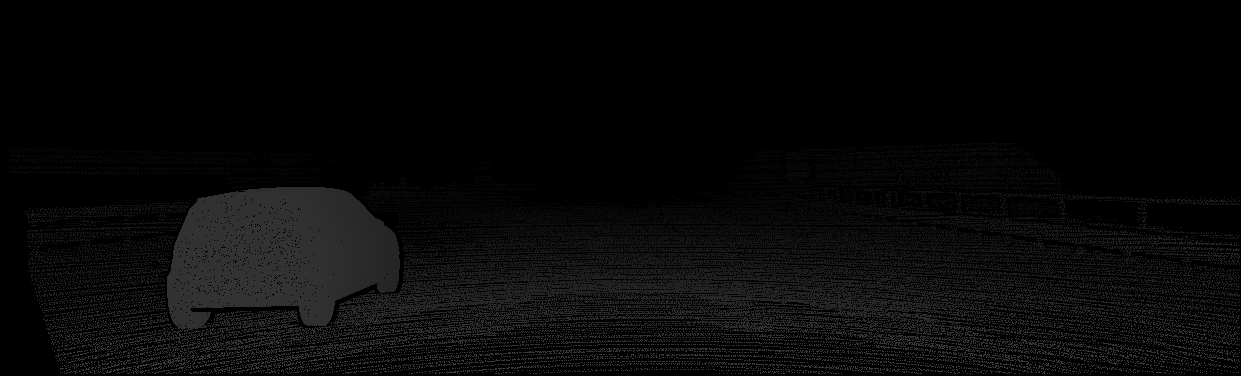
\includegraphics[width=13cm]{img/sgm_best_ground_truth.png}\label{fig:kitti-min-sgm-true-disparity}}

  \centering
  \subfloat[Pripadni izračunati dispariteti (16 smjerova)]{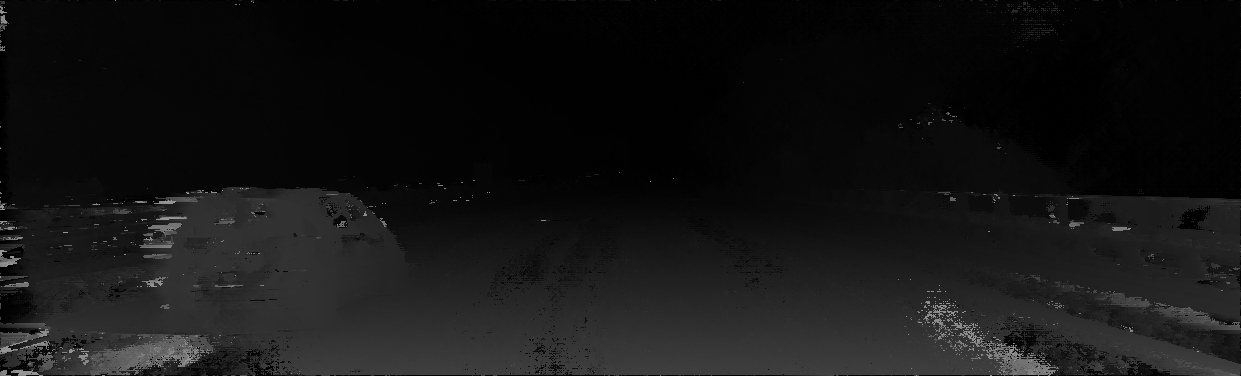
\includegraphics[width=13cm]{img/sgmbt_000188_10_150.png}\label{fig:kitti-min-sgm-calc-disparity}}

  \caption{Slika s najmanjom pogreškom uz korištenje SGM + BT u skupu KITTI}
\end{figure}

Slika s najgorim rezultatom u varijanti s 8 smjerova bila je {\verb|000169_10.png|} koja je prikazana na slici \ref{fig:kitti-max-sgm8-error}. Pogreška iznosi 57\%. Vidimo da slika ima puno objekata koji su
nepravilnog oblika što je dosta nepogodno za računanje korespondencije. Iz tog razloga rezultat na toj slici nije najbolji.

\begin{figure}[H]
  \centering
  \subfloat[Slika s najvećom pogreškom u skupu KITTI]{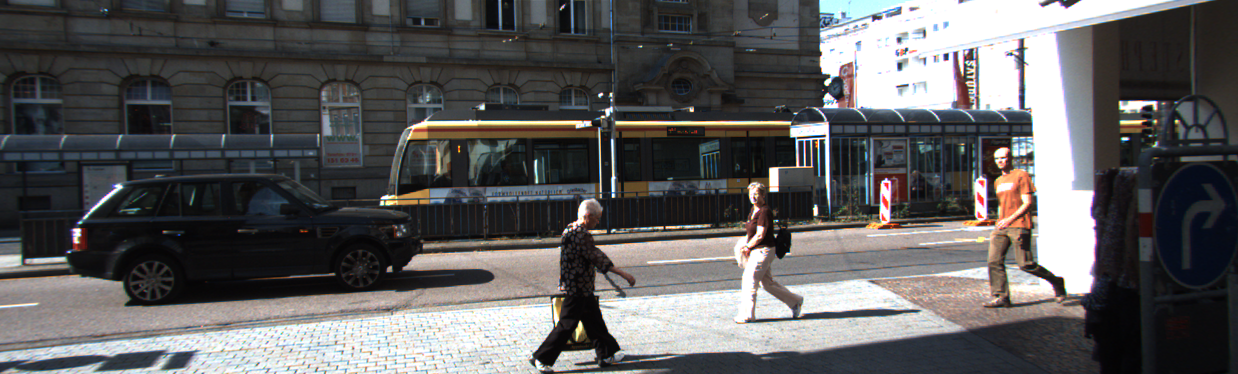
\includegraphics[width=13cm]{img/sgm_8_worst.png}\label{fig:kitti-max-sgm8-error}}
  
  \centering
  \subfloat[Pripadni točni dispariteti]{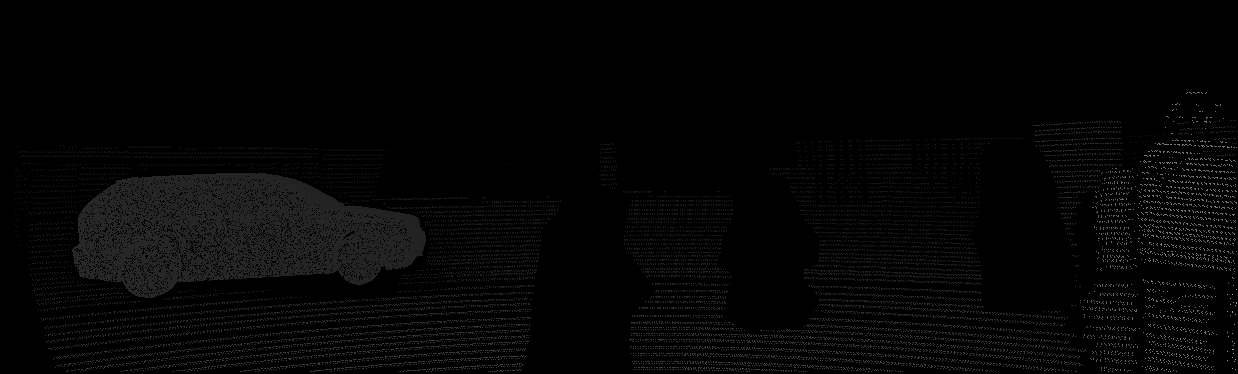
\includegraphics[width=13cm]{img/sgm_8_worst_ground_truth.png}\label{fig:kitti-max-sgm8-true-disparity}}

  \centering
  \subfloat[Pripadni izračunati dispariteti (8 smjerova)]{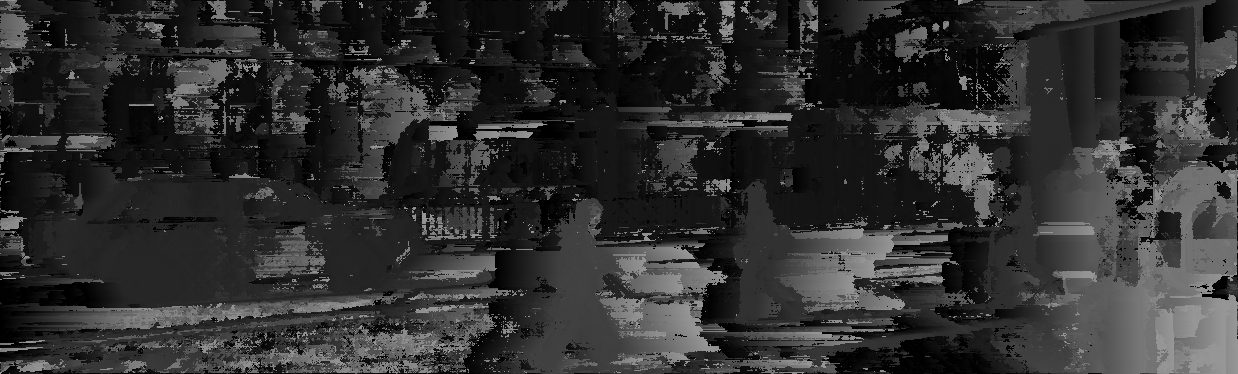
\includegraphics[width=13cm]{img/sgmbt_000169_10_150.png}\label{fig:kitti-max-sgm8-calc-disparity}}

  \caption{Slika s najvećom pogreškom uz korištenje SGM + BT u skupu KITTI (8 smjerova)}
\end{figure}

U varijanti sa 16 smjerova, slika s najvećom pogreškom bila je {\verb|000177_10.png|}, a
pogreška je iznosila 52\%. Na slici vidimo dosta izražen odbljesak sunca što može biti
razlog tako lošeg rezultata. Boljim uvidom utvrđeno je da je to slučaj te su priložene obje
slike za lakšu usporedbu. Vidimo da se razina osvjetljenja razlikuje na slikama što je
vrlo nepovoljan slučaj kod stereoskopske rekonstrukcije i dosta otežava postupak.

\begin{figure}[H]
  \centering
  \subfloat[Slika s najvećom pogreškom u skupu KITTI (lijeva)]{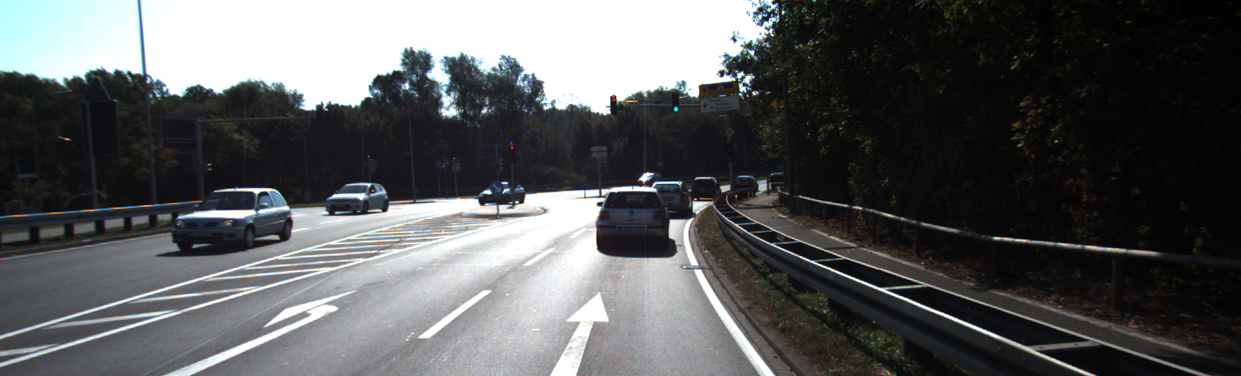
\includegraphics[width=13cm]{img/sgm_16_worst.png}\label{fig:kitti-max-sgm16-error_left}}

  \centering
  \subfloat[Slika s najvećom pogreškom u skupu KITTI (desna)]{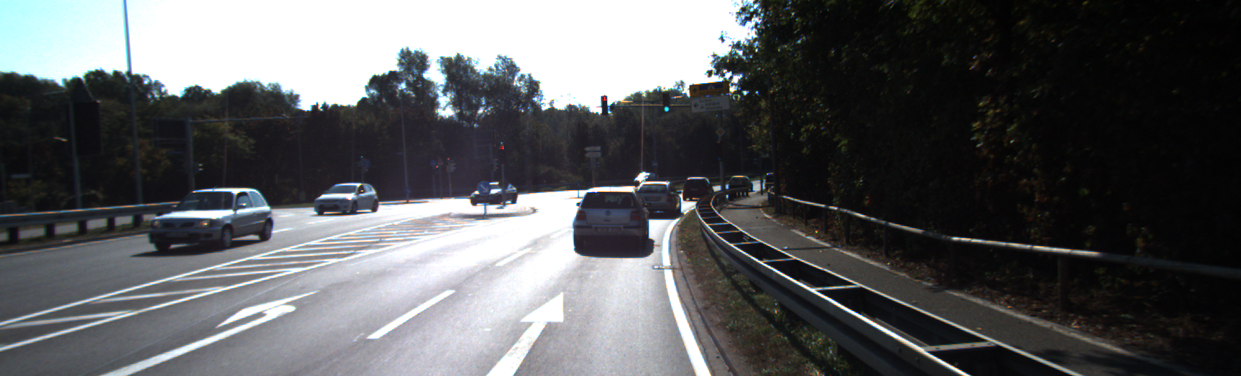
\includegraphics[width=13cm]{img/000177_10.png}\label{fig:kitti-max-sgm16-error_left}}
  
  \centering
  \subfloat[Pripadni točni dispariteti]{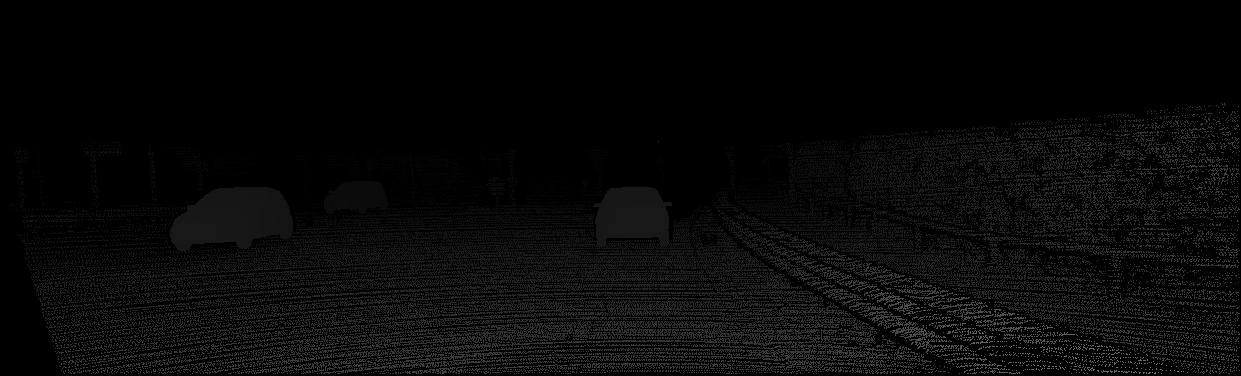
\includegraphics[width=13cm]{img/sgm_16_worst_ground_truth.png}\label{fig:kitti-max-sgm16-true-disparity}}

  \centering
  \subfloat[Pripadni izračunati dispariteti (16 smjerova)]{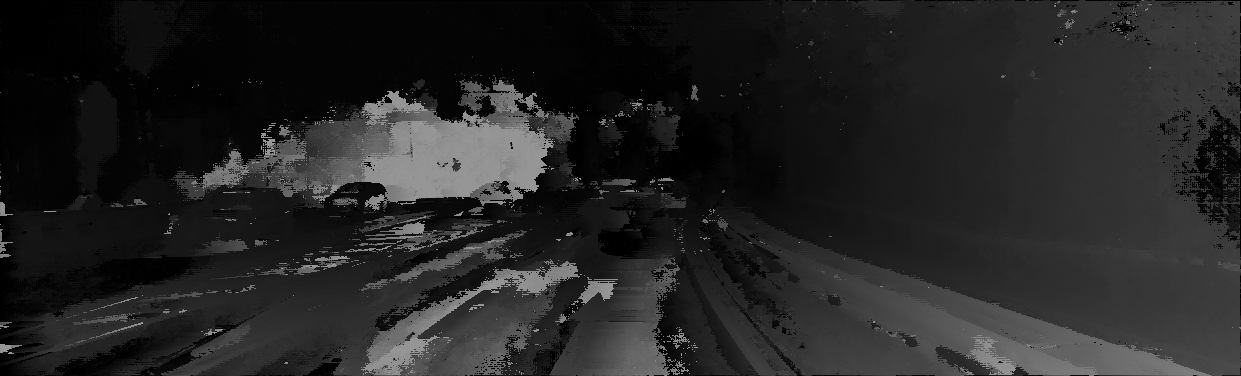
\includegraphics[width=13cm]{img/sgmbt_000177_10_150.png}\label{fig:kitti-max-sgm16-calc-disparity}}

  \caption{Slika s najvećom pogreškom uz korištenje SGM + BT u skupu KITTI (16 smjerova)}
\end{figure}

Prosječna pogreška u varijanti a 8 smjerova iznosila je 19.77\% dok je u varijanti sa 16
smjerova iznosila 17.97\%. Vidimo da razlika nije velika, ali je očekivano varijanta sa 16 smjerova bolja zbog bolje pokrivenosti cijele slike.

\chapter{Zaključak}
Cilj ovog rada bio je upoznati se s metodama guste stereoskopske rekonstrukcije, s naglaskom
na poluglobalno podudaranje. Prvo su obrađene metode lokalne korespondencije koje se temelje
na principu prozorčića. Zatim je uveden algoritam poluglobalnog podudaranja koji kao ulaz
prima cijene izračunate kod lokalnih metoda. Njegova ideja je da optimira globalnu funkciju energije na način da preferira glatkoću površina, a kažnjava prekide u kontinuitetima.
Navedeni algoritmi su testirani na standardnim skupovima slika Middlebury i KITTI, a rezultati
su uglavnom u skladu s očekivanim. Jedino iznenađenje bila je metoda Census u kombinaciji sa poluglobalnim podudaranjem koja je dala izrazito dobre rezultate.

Kao sljedeći korak u poboljšanju navedenih metoda mogle bi se implementirati visoko paralelizirane verzije algoritama
koje bi se izvodile na grafičkim karticama. Osim toga, moguće je implementirati i dodatne
korake u algoritmu poluglobalnog podudaranja koji bi ostvarili još bolje rezultate, poput
uklanjanja naglih skokova u disparitetu (eng. {\sl peaks}), zaglađivanja Gaussovim filtrom i tako dalje.

\bibliography{literatura}
\bibliographystyle{fer}

\begin{sazetak}
  Ovaj rad razmatra metode guste stereoskopske rekonstrukcije na standardnim skupovima slika.
  Cilj takvih metoda je odrediti oblak točaka koji najbolje odgovara prostoru projiciranom
  na slici.
  Poseban naglasak je na metodama koje favoriziraju glatku rekonstrukciju. Kao glavni
  algoritam uvedeno je poluglobalno podudaranje koje se temelji na pretpostavci da radimo
  uglavnom s glatkim površinama. Zato algoritam kažnjava svaki prekid u dubini slike. Kao
  ulaze prima cijene izračunate u metodama lokalne korespondencije. Algoritmi su
  evaluirani na standardnim skupovima slika Middlebury i KITTI. Rezultati i usporedbe metoda su prikazani
  grafički i komentarima.

\kljucnerijeci{računalni vid, stereoskopska rekonstrukcija, poluglobalno podudaranje, disparitet, korespondencija}
\end{sazetak}

\engtitle{Dense stereoscopic reconstruction with semi-global matching}
\begin{abstract}
  This thesis considers methods for dense stereoscopic reconstruction on standard image
  datasets. The aim of such methods is to determine the cloud of points that best suits
  the space projected onto the picture.
  Particular emphasis is placed on methods that favor smooth reconstruction. As the main
  algorithm, the thesis introduces semi-global matching which is based on the assumptions
  that we are mainly concerned about smooth surfaces. That is the reason why the algorithm
  penalizes every discontinuity in the depth of the image. It accepts, as input, the costs
  calculated by local correspondence methods. Algorithms are evaluated on standard image
  datasets Middlebury and KITTI. Results and comparisons of the methods are shown graphically
  and discussed.
  
\keywords{computer vision, stereoscopic reconstruction, semi-global matching, disparity, correspondence}
\end{abstract}

\end{document}
